\UseRawInputEncoding
\documentclass[class=article,crop=false]{standalone}
\usepackage{pacco}
\begin{document}
\section{Markov Chains}
\subsection{Overview}
%\tikzexternalize
Let ($\Omega, \mathscr{F}, \mathbb{P}$) be a probability space. Then, a \enf{stochastic process} is a collection 
\[\{X(t,\omega), \; t\in T\}\]
of random variables
\[X:T\times\mathscr{F} \longrightarrow S\]
where:
\begin{itemize}
    \item $T$ is the \sott{index set} (typically interpreted as time); 
    \begin{example}
        $T:= \mathbb{Z}_+=\{0,1,2,\ldots\}$: $T$ is a \textit{discrete time} ($\{X_n, \; n\in\mathbb{Z}_+\}$).
    \end{example}
    \begin{example}
        $T:=\mathbb{R_+}$:$T$ is a \textit{continuous time}.
    \end{example}
    \item $S$ is the \sott{state space}. $S$ can be countable: we can take $S \subseteq \mathbb{Z}$ and denote the elements of $S$ as $i, j, k, \ldots$ or $i_1, i_2, i_3, \ldots$.
\end{itemize}
If $X_n=i$ we say that $X$ is in state $i$ or that $X$ visits $i$ at time $n$. Typically we drop the argument $\omega$ in $X(t,\omega)$ and just write $X(t)$. $X(\cdot,\omega)$ for a fixed $\omega$ is a function of $t$ and is called \sott{trajectory} of $X$.

More generally one could have:
\begin{itemize}
    \item $T \subset \mathbb{R}^d$: \textbf{random fields} (e.g. geographical coordinates: $X$ is a pair of latitude and longitude data and the state is the height data $\rightarrow T \subset \mathbb{R}^2$);
    \item $S \subset \mathbb{R}$;
    \item $S \subset \mathbb{R}^d$: \textbf{multivariate processes};
\end{itemize}

\begin{definition}
    A \enf{Markov Chain} (MC) is a discrete-time stochastic process $\{X_n,n\in\mathbb{Z}_+\}$ taking values in a countable space $S$, such that:
    \begin{align}\label{markprop}
        &\prob(X_n=i_n|X_0=i_0,\ldots,X_{n-1}=i_{n-1})\\
        =&\prob(X_n=i_n|X_{n-1}=i_{n-1})\qquad\forall n\,\geqslant1,\;\forall\,i_0,\ldots,i_n \in S.
    \end{align}
    This property is called \enf{Markov property.}
\end{definition}
Markov property defines a very broad class of Markov process es. Given the current state $X_{n-1}$, the next $X_n$ does not depend on the state previous to $n-1$. We could express these concepts in terms of $\sigma$-algebras and filtrations: if
\[
\mathscr{F}^x_n=\sigma(x_k, k\leqslant n)
\]
and 
\[
\{\mathscr{F}^x_n,n\in \mathbb{Z}_+\}
\]
is the natural filtration, the previous reads:
\[
\prob(X_n=i_n|\mathscr{F}^x_{n-1})=\prob(X_n=i_n|X_{n-1}).
\]
$\mathscr{F}^x_{n-1}$ renders useless the information previous to $n-1$.\bigskip\\
From what we studied in our earlier courses, the main assumption in classical inference was the fat that the samples were i.i.d. But at a certain point we need a more sophisticated model that gives up this assumption. If the data are not i.i.d. we need to make a choice regarding the dependence between the data. Markov processes are highly studied because they offer a way of mathematically studying the dependence between samples (another common way is recurring to \textit{Bayesian inference}). 
\begin{remark}
    The Markoviality is one way of departing from i.i.d. assumptions and all results that follow come from this property.
\end{remark}
The dyamics of $X$ are specified therefore by the right hand side of the Markov Property equation \ref{markprop}
\[p_{ij}=\prob(X_{n+1}=j|X_n=i)\]
which is called \enf{transition probability}.\\
We will assume that these are \sott{temporary homogeneous}, i.e. they do not depend on time. So we can denote
\[p_{ij}=\prob(X_{n+1}=j|X_n=i) \]
for any time $t$. We call $j$ the \textit{arrival state} ad $i$ the \textit{starting state}.
\begin{remark}
    \sott{Spatial homogeneity} is a much stronger assumption, not made here in general. In this case, $p_{ij}$ only depends on $j$: $p_{ij}=p_{0, j-1}$. For example, if we analyzed the probability of moving between the tiles of a grid, spatial homogeneity would imply that moving from one tile to another is the same regardless to the starting tile.
\end{remark}

We tipically collect the $p_{ij}$ in a \enf{transition matrix}:
\[P=(p_{ij}) \; i,j\in S\]
\begin{example}
    For $S=\{0,1,\ldots,k\}$ we have:\\
    \[\begin{bmatrix} 
    p_{00} & p_{01} & \dots & p_{0k} \\
    \vdots & \ddots&  & \vdots \\
    \vdots &  & \ddots & \vdots \\
    p_{k0} & p_{k1} & \dots & p_{kk}
\end{bmatrix}\]
\end{example}
P is a \sott{stochastic matrix} since:
\begin{itemize}
    \item $p_{ij}\geqslant 0\qquad \forall\; i,j \in S$;
    \item $\forall \;i \in S: \qquad \sum_{j\in S}p_{ij}=1$.
\end{itemize}
Now $i$ is then the conditional distribution of $X_{n+1}$ given $X_n=i$.\\
We typically use a graph to represent a MC.
\begin{example}
    \[
    P=\begin{bmatrix} 
    p_{00} & p_{01} & 0 \\
    p_{10} & 0 & p_{12} & \\
    0 & p_{21} & 0
\end{bmatrix}
    \]
    
\begin{figure}[H]
    \centering
    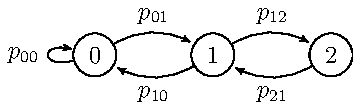
\includegraphics{../standalones/pdfs/simplechain.pdf}
    \label{sonoebreo}
\end{figure}
\end{example}
Is the transition matrix enough to derive everything about the Markov process? In other words, does the transition matrix \sott{fully characterize} the distribution and the features of the process? The answer is yes but only if we include the \enf{initial distribution} of the chain.

\begin{definition}
    Define the \enf{initial distribution} of the chain
    \[
    \lambda_i=\prob(X_0=i)\qquad i\in S
    \]
    as the law of the starting state. 
\end{definition}
If \[\lambda_i=\delta_{ij}\footnote{Kronecker's delta.} =
\begin{cases}
    1,& \text{if } i=j\\
    0,              & \text{otherwise}
\end{cases}\]
then $X_0=j$ almost surely.

\begin{proposition}
    Let $X$  be a MC on $S$ countable with initial distribution $\lambda=i \in S$ and transition matrix P. Then $\lambda$ and $P$ jointly fully charcterize the law of the chain. 
\end{proposition}
\begin{proof2}
    What do we need to prove? We need to examine the joint distribution of a Markov Chain, which is an infinite sequence of random variables that are not i.i.d.: we can't therefore write the joint distribution as the product of the single distributions.

    We need to show that $(\lambda, P$) allows us to compute all joint distributions for the chain, i.e. $\forall$ choices of $0\leqslant j_1 < j_2 < \ldots < j_k$ the law $\prob(X_{j_1}=i_{j_1}, \ldots, X_{j_k}=i_{j_k})$\footnote{This is called a \sott{projection}: we are projecting an infinite sequence on a finite subset.}, which has $k$ states, can be computed with $(\lambda, P$) only. We can use the previous as the marginal of the joint distribution for times $0, \ldots, j_k$:
    \[
    \underbrace{0,1,\dots,j_{1-1}}_{\mathclap{\text{marginalize}}},\textcolor{RedViolet}{j_1},\underbrace{j_{1+1},\ldots}_{\mathclap{\text{marginalize}}},\textcolor{RedViolet}{j_2},\underbrace{\ldots}_{\mathclap{\text{marginalize}}},\textcolor{RedViolet}{j_k}
    \]
    i.e. it is
    \[
    \sum_{\underbrace{i_h\in S | h \neq j_1,\ldots,j_k}_\text{indices of times not chosen: $h \in \{o, \ldots, j_k\}$}} \prob(\underbrace{X_0=i_0, X_1=i_1,\ldots,X_{j_1}=i_{j_k}}_\text{$j_k + 1$ states})
    \]
    So it is enough to find $\prob(X_0=i_0,\ldots,X_n=i_n)$, but by the chain rule this equals to 
    \[\prob(X_0=i_0,\ldots,X_{n-1}=i_{n-1}) \cdot \prob(X_n=i_n|X_0,\ldots,X_{n-1})\]
    and thanks to Markov Property this is equal to
    \begin{align*}
           &\prob(X_0=i_0,\ldots,X_{n-1}=i_{n-1}) \cdot p_{i_{n-1},i_n}\\
           =&\ldots=\underbrace{\prob(X_0=i_0)}_{\lambda_{i_0}}\cdot       p_{i_0,i_1}\cdot\ldots\cdot p_{i_{n-1},i_n}
    \end{align*}
    So we only need $\lambda_{i_0}$ and the $P$ matrix.
\end{proof2}

We can use a compact notation (took from Norris textbook)
\[X \sim \text{Markov}(\lambda,P).\]

\begin{definition}
  We define the \enf{$k$-step transition probabilities} as
\begin{align*}
    &p_{ij}^{(k)} := \prob(X_{n+k}=j|X_n=i), \qquad k \in \mathbb{N}\\
    &p_{ij}^{(0)} := \delta_{ij} = \begin{cases}
        1 & i=j\\
        0 & \text{else}
    \end{cases}
\end{align*}
\end{definition}

\begin{proposition}{\enf{Chapman-Kolmogorov equations:}}
    for all $e$, $m \in \mathbb{Z}_+$
    \begin{equation}\label{chapkolm}
        p_{ij}^{(e+m}=\sum_{k<j}p_{ik}^{(e)}\cdot p_{kj}^{(m)}
    \end{equation}
\end{proposition}
The proof is left as exercise (use graphical intuition below: marginalize out unwanted states and use Markov property). 
\begin{figure}[H]
    \centering
 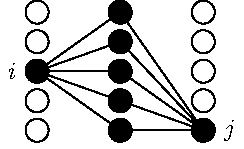
\includegraphics{../standalones/pdfs/marginchain}
    \label{mc graph} %porcoddio sono un cazzo di dragooOOO
\end{figure}

If you take the transition matrix to the power of $k$, $P^k$ is still a stochastic matrix and the entries are $p_{ij}^(k)$.
\begin{example}
    \begin{figure}[H]
    \centering
    \begin{tikzpicture}[->,>=stealth',shorten >=2pt, line width=0.5pt, node distance=2cm]
        \node [circle, draw] (zero) {0};
        \node [circle, draw] (one) [right of=zero] {1};
        \path (zero) edge [bend left] node [above] {$\alpha$} (one);
        \path (zero) edge [loop left] node [left] {$1-\alpha$} (zero);
        \path (one) edge [loop right] node [right] {$1-\beta$} (zero);
        \path (one) edge [bend left] node [below] {$\beta$} (zero);
    \end{tikzpicture}
    \label{sadasdasf}
\end{figure}
\[
P^2=P\cdot P=\ldots=\begin{bmatrix}
    p_{00}^{(2)} & p_{01}^{(2)}\\
    p_{10}^{(2)} & p_{11}^{(2)}
\end{bmatrix}
\]
In this case, the intermediate states don't matter. For instance we have $p_{00}^{(2)}=p_{00}p_{00}+p_{01}p_{10}$
\end{example}
\subsection{Notable Markov processes}
\subsubsection*{Random Walk}
Given $X_0$, the simple random walk is defined as
\[X_n=X_{n-1}+Y_n\]
$Y_n$s are i.i.d.:
\[
Y_n=\begin{cases}
    1 &\text{with probability}\; p\\
    -1 &\text{with probability}\; 1-p
\end{cases}
\]
\[
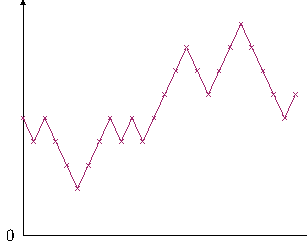
\includegraphics{../standalones/pdfs/simplerw}
\]
if $p=\frac{1}{2}$ the the random walk is \sott{symmetric}.\\
Random walks have application, for instance, in:
\begin{itemize}
    \item approximation of Brownian motion and other diffusion processes useful in:
    \begin{itemize}
        \item physics;
        \item math finance;
        \item math biology;
    \end{itemize}
    \item random explorations of space:
    \begin{itemize}
        \item Monte-Carlo integration (Monte-Carlo Markov Chain methods);
        \item stochastic optimization
        \item integral approximation
    \end{itemize}
\end{itemize}
Some possible extensions are:
\begin{itemize}
    \item changing the state space dimension: imagine a symmetric random walk in $\mathbb{Z}^d$, $i,j \in \mathbb{Z}^d$ with $i=(i_1,\ldots,i_d)$:
    \[
    p_{ij}=\begin{cases}
        \frac{1}{2d} & \text{if}\quad \sum_{k=1}^q|i_k-j_k|=1\\
        0 & \text{else;}
    \end{cases}
    \]
    \item change law of $Y_n:\prob(Y_n=1)=a_i, \; \in \mathbb{Z}$ (the case of the distribution being heavy tailed is particularly interesting);
    \item change the topology of $S$:
    \begin{itemize}
        \item Random walk on manifold sphere, on torus...;
        \item Random walk on graphs; for example choose uniformly with probability $q$ a node in the graph (Google PageRank Algorithm).
    \end{itemize}
\end{itemize}
\subsubsection*{Birth-and-death chains}
We define the transition probabilities as
\[
p_{ij}=\begin{cases}
    p_i & j=i+1\\
    1-p_i & j=(i-1)^+\\
    0 &\text{else}
\end{cases}
\]
\begin{figure}[H]
    \centering
    \begin{tikzpicture}[->,>=stealth',shorten >=2pt, line width=0.5pt, node distance=2cm]
        \node [circle, draw] (zero) {0};
        \node [circle, draw] (one) [right of=zero] {1};
        \node [circle, draw] (two) [right of= one] {2};
        \node [circle, draw] (dots) [right of=two] {$\ldots$};
        \path (zero) edge [bend left] node [above] {$p_0$} (one);
        \path (zero) edge [loop left] node [left] {$1-p_0$} (zero);
        \path (one) edge [bend left] node [below] {$1-p_1$} (zero);
        \path (one) edge [bend left] node [above] {$p_1$} (two);
        \path (two) edge [bend left] node [above] {$p_2$} (dots);
        \path (dots) edge [bend left] node [below] {} (two);
        \path (two) edge [bend left] node [below] {$1-p_2$} (one);
    \end{tikzpicture}
    \label{ahah}
\end{figure}
\begin{itemize}
    \item Time-varying size of a population (animal, viruses, numbero of request to a CPU...)
    \item size of a queue at a server
    \item dimension of a multivariate distribution used for estimation
    \item dimension $k$ of a mixture model
    \[
    \text{i.e.} \qquad \sum_{i=k}^k w_i f_i
    \]
    with $\sum_{w_i}=1$ and $f_i$ being a density.
\end{itemize}
\subsubsection*{Pòlya urns}
An urn contains $W_0$ white balls and $B_0$ black a ball. We draw a ball, check its colour, put it back and add to the urn another ball of the same colour: this behaviour is called \sott{reinforcement} and it is the opposite of drawing without placement. Let $W_n$ be the number of white balls after n draws (steps):
\[
\prob(W_{n+1}=j|W_0,\ldots,W_n)=\begin{cases}
    \frac{W_n}{Wn+Bn}\rightarrow\text{"draw white"} &j=W_n+1\rightarrow\text{"add white"}\\
    \frac{B_n}{Wn+Bn}\rightarrow\text{"draw black"} &j=W_n\rightarrow\text{"same number of whites"}\\
    0 & \text{else}
\end{cases}
\]
\begin{align*}
    W_n+&B_n=W_0+B_{0+n}\\
    &B_n=W_0+B_{0+n}-W_n
\end{align*}
The probability only depends on $W_n$ and the previous $W$s are irrelevant, so the process is a Markov Chain
These are applied in Bayesian inference, since they generate \sott{exchangeable sequences} ($(X_1, X_2)\stackrel{d}{=}(X_2,X_1)$). A classical result which is often used is:
\[
\frac{W_n}{W_n+B_n}\xrightarrow{a.s}\theta\sim Beta(W_0, B_0)
\]
\subsubsection*{Branching Processes}
Branching processes are a simple model for evolving populations with reproduction. The basic formulation (Galton-Watson) is:
\begin{itemize}
    \item individuals live on period;
    \item individuals generate clones independently (the original motivation was the survival of family names);
    \item the next generation is formed by the offspring of the previous generation.
\end{itemize}

\begin{figure}[H]
    \centering
    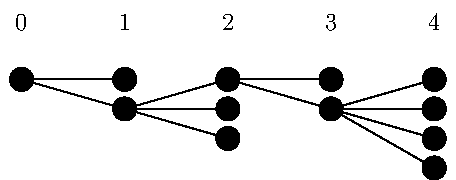
\includegraphics{../standalones/pdfs/bp}
    \label{generatons}
\end{figure}
Useful applications:
\begin{itemize}
    \item epidemiology (virus contagion);
    \item population genetics;
    \item physics (random number of neutron produced at collisions).
\end{itemize}
Interesting extensions:
\begin{itemize}
    \item extend to $k$ types;
    \item add immigration.
\end{itemize}
Let $X_n$ be the number of individuals in generation $n$ and $Y_i$ be the number of clones/offspring of individual $i$. We have $Y_i \stackrel{i.i.d.}{\sim} p_Y$ on $\mathbb{Z}_+$.
\[
X_n=Y_1+Y_2+\ldots+Y_{X_{n-1}}=\sum_{i=1}^{X_{n-1}}Y_i\independent X_{n-2},X_{n-3},\ldots
\]
So the process is a Markov chain. 

\begin{proposition}{\enf{Branching Property:}}
    Denote by $X^{(i)}=\{{X_n}, n \in \mathbb{Z}_+|X_0=1\}$, characterizing the chain by a fixed starting point, the branching process started at $i$. Let $\Tilde{X},\hat{X}$ be independent copies of $X$. Then
    \begin{equation}
        X^{(i+j)}\stackrel{d}{=}\Tilde{X}^{(i)}+\hat{X}^{(j)}
    \end{equation}
    This is called \enf{branching property}.
\end{proposition}
\begin{proof2}
    Let 
    \[
    g_{z}(s)=\ev{e^{sZ}}
    \]
    be the moment generating function of $Z$. We are interested in the moment generating function of $X_1|X_0=i$.
    \begin{align*}
       g_{X_1^{(i)}}=g_{\sum_{j=1}^{i}Y_j} =(g_Y)^i
    \end{align*} 
    This moment generating function characterizes the one step transition probability of getting to $X_1$, that is the population size at $n=1$, from the state $X_0=i$. Now
    \begin{align*}
         &g_{\{\Tilde{X}_1^{(i)}+\hat{X}_1^{(j)}\}}=g_{\Tilde{X}_1^{(i)}}\cdot g_{\hat{X}_1^{(j)}}=\\
         =(&g_Y)^i\cdot(g_Y)^j=(g_Y)^{i+j}=g_{X_1^{(i+j)}}
    \end{align*}
    We have now proved for one step that, since $\Tilde{X}_1^{(i)}+\hat{X}_1^{(j)}$ and $X_1^{(i+j)}$ share the same moment generating function, they have the same distribution. To extend this result to every step we can use Markov property, so that $X^{(i+j)}_1\stackrel{d}{=}\Tilde{X}^{(i)}_1+\hat{X}^{(j)}_1$ characterizes the law of the entire chain.
\end{proof2}
An interesting extension of the model consists in the behaviour of a population during extinction. This ultimately depends on:
\[
\ev{Y}=\begin{cases}
    <1 & X\; \text{is subcritical}\\
    =1 & X\; \text{is critical}\\
    >1 & X\; \text{is supercritical}\\
\end{cases}
\]
An interesting case is given by introducing immigration to the subcritical case. This is called \enf{Galton-Watson} branching process.
\subsubsection*{Wright-Fisher models}
These model the time-varying frequency of 2 types (in general k or $\infty$ many types) in an evolving population of constant size. The original motivation was modelling the allelic type frequency of a gene locus. These models have the following characteristics:
\begin{itemize}
    \item individuals live 1 period;
    \item individuals can be of type 0 or 1;
    \item population size is $N$ $\forall n \geqslant \mathbb{Z}_+$;
\end{itemize}

\begin{figure}[H]
    \centering
    \begin{tikzpicture}[-,>=stealth', line width=0.5pt, node distance=0.5cm]
        \node [circle] (zero) {0};
        \node [circle, draw, shade, shading=ball, circle, ball color=RedViolet!80!white] (a) [below=0.4cm of zero]{};
        \node [circle, draw, shade, shading=ball, circle, ball color=RedViolet!80!white] (b) [below of= a]{};
        \node [circle, draw, shade, shading=ball, circle, ball color=RedViolet!80!white] (c) [below of= b]{};
        \node [circle, draw, shade,shading=ball,circle,ball color=Dandelion!80!white] (d) [below of= c]{};
        
        \node [circle] (one)[right=1cm of zero] {1};
        \node [circle, draw, shade, shading=ball, circle, ball color=RedViolet!80!white] (e) [below=0.4cm of one]{};
        \node [circle, draw, shade, shading=ball, circle, ball color=RedViolet!80!white] (f) [below of= e]{};
        \node [circle, draw, shade,shading=ball,circle,ball color=Dandelion!80!white] (g) [below of= f]{};
        \node [circle, draw, shade,shading=ball,circle,ball color=Dandelion!80!white] (h) [below of= g]{};
        
        \node [circle] (two)[right=1cm of one] {2};
        \node [circle, draw, shade, shading=ball, circle, ball color=RedViolet!80!white] (i) [below=0.4cm of two]{};
        \node [circle, draw, shade, shading=ball, circle, ball color=RedViolet!80!white] (j) [below of= i]{};
        \node [circle, draw, shade, shading=ball, circle, ball color=RedViolet!80!white] (k) [below of= j]{};
        \node [circle, draw, shade,shading=ball,circle,ball color=Dandelion!80!white] (l) [below of= k]{};        
        \node [circle] (three)[right=1cm of two] {3};
        \node [circle, draw, shade, shading=ball, circle, ball color=RedViolet!80!white] (m) [below=0.4cm of three]{};
        \node [circle, draw, shade,shading=ball,circle,ball color=Dandelion!80!white] (n) [below of= m]{};
        \node [circle, draw, shade,shading=ball,circle,ball color=Dandelion!80!white] (o) [below of= n]{};
        \node [circle, draw, shade,shading=ball,circle,ball color=Dandelion!80!white] (p) [below of= o]{};

        \path (a) edge node [below] {} (e);
        \path (a) edge node [below] {} (f);
        \path (d) edge node [below] {} (g); 
        \path (d) edge node [below] {} (h); 

        \path (e) edge node [below] {} (i); 
        \path (e) edge node [below] {} (j); 
        \path (e) edge node [below] {} (k); 
        \path (h) edge node [below] {} (l); 

        \path (j) edge node [below] {} (m); 
        \path (l) edge node [below] {} (n); 
        \path (l) edge node [below] {} (o); 
        \path (l) edge node [below] {} (p); 
    \end{tikzpicture}
    \label{wright models}
\end{figure}
We have now constrained the population size, so each parent can generate from 0 to $N$ offspring and therefore birth events are no longer independent. A useful approach to model this behaviour is to imagine that during next generation individuals choose their parent at random from the previous generation, with the condition that it must be of the same type.\\
Let $X_n$ be the number of type-0 individuals at time $n$. The individuals at generation $n$ are:
\begin{itemize}
    \item of type-0 with probability $\frac{X_n}{N}$;
    \item of type-1 with probability $1-\frac{X_n}{N}$;
\end{itemize}
So every member of a generation chooses its parent by a Bernoulli trial \sott{independently}. Since we have $N$ Bernoulli trial with parameter $p=\frac{X_n}{N}$, we have that:
\[
X_n|X_{n-1}\sim Binom(N,\frac{X_{n-1}}{N}).
\]
Note that 
\begin{align*}
    \text{if}\quad &X_{n-1}=0 \implies X_n=0\qquad\text{a.s}\\
    \text{if}\quad &X_{n-1}=N \implies X_n=N\qquad\text{a.s}.
\end{align*}

\begin{figure}[H]
    \centering
        \begin{tikzpicture}
            \begin{axis}[
                xlabel=0,
                every axis x label/.style={
                at={(ticklabel* cs:-0.01)},
                anchor=east,
            },
                ylabel=\empty,
                xmin=0, xmax=52,
                ymin=0, ymax=100,
                axis y line=left,
                y axis line style={opacity=0},
                ytick=\empty,
                xtick={46}, 
                xtick style={draw=black}, 
                xticklabel={fixation event}, 
                axis x line*=bottom
                        ]
                \addplot[mark=x,RedViolet] plot coordinates {
                    (0,50)
                    (2,40)
                    (4,50)
                    (6,40)
                    (8,30)
                    (10,20)
                    (12,30)
                    (14,40)
                    (16,50)
                    (18,40)
                    (20,50)
                    (22,40)
                    (24,30)
                    (26,20)
                    (28,30)
                    (30,40)
                    (32,30)
                    (34,20)
                    (36,10)
                    (38,20)
                    (40,10)
                    (42,20)
                    (44,10)
                    (46,0)
                    (48,0)
                    (50,0)
                };
                %\node[below,RedViolet,align=left] at (46,-0.08) {\footnotesize fixation event};
            \end{axis}
                \begin{axis}[
                xlabel=$N$,
                    every axis x label/.style={
                at={(ticklabel* cs:-0.01)},
                anchor=east,
            },
                ylabel=\empty,
                xmin=0, xmax=30,
                ymin=0, ymax=100,
                axis y line=left,
                y axis line style={opacity=0},
                ytick=\empty,
                xtick=\empty,
                axis x line*=top]
            \end{axis}
    \end{tikzpicture}
    \label{camminata}
\end{figure}
Some useful extension may include:
\begin{itemize}
    \item mutations;
    \item $k\leqslant\infty$ types;
    \item uncountably many types.
\end{itemize}
For example, set mutations such that they only occur to the other type:
\[
\alpha=\prob(1\rightarrow0)\qquad\beta=\prob(0\rightarrow1).
\]
Mutations take place before reproduction (that is, before the binomial resampling method). We have:
\begin{itemize}
    \item a $Bernoulli(\beta)$ trial on each of $i$ individual of type 0. On average:
    \begin{itemize}
        \item $i\beta$ individuals become of type 1;
        \item $i(1-\beta)$ individuals remain of type 0;
    \end{itemize}
    \item a $Bernoulli(\alpha)$ trial on each of $N-i$ individual of type 1. On average:
    \begin{itemize}
        \item $(N-i)\alpha$ individuals become of type 0;
        \item $(N-i)(1-\alpha)$ individuals remain of type 1.
    \end{itemize}
\end{itemize}
After mutation, the expected proportions are:
\begin{alignat*}{3}
    &\text{type 0:}&&\qquad \Tilde{p_i}&&=\frac{1}{N}(i(1-\beta)+(N-i)\alpha)=\\
    & && &&=\frac{i}{N}(1-\beta)+(N-i)\alpha=\\
    & && &&=p_i(1-\beta)+(1-p_i)\alpha.\\
    \\
    &\text{type 1:}\qquad &&1-\tilde{p_i}&&=p_i\beta+(1-p_i)(1-\alpha).
\end{alignat*}
We can interpret $\tilde{p}_i$ as the \sott{percentage} of type 0 individuals (in expectation) before resampling. The transition probability has become:
\[=0
p_{ij}=\prob(X_{n+1}=j|X_n=i)=\binom{N}{j}\Tilde{p}_i^j(i-\Tilde{p}_i)^{N-j}
\]
Now, if $i=0\implies p_i=\frac{i}{N}=0\implies\Tilde{p}_i=\alpha\implies\prob(X_{n+1}>0|X_n=0)=1-(1-\alpha)^N>0$.\\
If $X_n$ is at the boundary $X_n \in \{o,N\}$, now there is positive probability of going back to the interior of the space state.
\subsubsection*{Transformation of Branching Processes}
Intuitively, there are two branching processes embedded in the Wright-Fisher trajectory. We can formalize this connection:

\begin{proposition}
    Let $X$ and $W$ be two independent branching processes with the same Poisson offspring distribution. Then, conditional on the total population size being constant and equal to $N$, $X$ and $W=N-X$ are Wright-Fisher chains.
\end{proposition}
\begin{proof2}
    \begin{align*}
        X_n&=\text{n° of type 0 individuals}\\
        W_n&=\text{n° of type 1 individuals}\\
    \end{align*}
    With per capita offspring
    \[
    Y\sim Pois(\lambda_j) \qquad j=0,1
    \]
    where $j$ is specific to the first and to the second branching process. Now, since the sum of Poisson variables is still a Poisson variable,
    \begin{align*}
        X_n &= \sum_{i=1}^{X_{n-1}}Y_i \sim Pois(X_{n-1}\lambda_0)\\
        W_n &= \sum_{i=1}^{W_{n-1}}Y_i \sim Pois(W_{n-1}\lambda_1)\\
    \end{align*}
    We know, in general, that
    \[
    Z_j\sim Pois(\gamma_j),\;j=0,1 \implies Z_0|Z_0+Z_1=N\sim Binom\biggl(N,\frac{\gamma_0}{\gamma_0+\gamma_1}\biggr)
    \]
    Let's apply this property:
    \[
    X_n|X_n+W_n=N,X_{n-1},W_{n-1}\sim Binom(N,q_{n-1})
    \]
    What we expect is for the parameter $q_{n-1}$ to only depend on state $n-1$. We know that:
    \[
    q_{n-1}=\frac{X_{n-1}\lambda_0}{X_{n-1}\lambda_0+\underbrace{W_{n-1}}_{\mathclap{N-X_{n-1}\;\text{because we are conditioning on the whole population}}}\lambda_1}=\frac{X_{n-1}\lambda_0}{X_{n-1}(\lambda_0-\lambda_1)+N\lambda_1}
    \]
    But we said that the offspring distribution is the \textit{same} Poisson distribution: so
    \begin{align*}
        &\lambda_0=\lambda_1\implies q_{n-1}=\frac{X_{n-1}}{N}\\
        \implies &X_n|X_{N-1},X_n+W_n=N \sim Binom\biggl(N,\frac{X_{n-1}}{N}\biggr)
    \end{align*}
    which is the transition probability of the Wright-Fisher chains, which characterizes the law of the entire chain. We are therefore claiming that the random variables whose state space is the $\infty$ trajectories of the chain is governed by one law.
\end{proof2}
\subsection{Review of Markov Property}
The property we gave that the beginning can be seen as a regeneration property:
\[
X\sim Markov(\lambda,P) \implies \{X_{n+k},k\geqslant 0|X_n=i\}\sim Markov(\delta_i,P).
\] 
Here $n$ is fixed and from $n$ onward the chain starts afresh with the same properties. What if $n$ is a random variable $T$, indicating a random time?

\begin{definition}{\enf{strong Markov property:}}
    We are interested in establishing the \enf{strong Markov property}:
    \begin{equation}
        \prob(X_{T+1}=j|X_0,\ldots,X_T=i)=\prob(X_{T+1}=j|X_T=i)
    \end{equation}
\end{definition}
Not all random times are suitable: let $\{\mathscr{F}\}_{n\geqslant 0}$ be the \sott{natural filtration} generated by $X$, where $\mathscr{F}_n=\sigma(X_u, 0\leqslant u \leqslant n)$ which is interpreted as the \textit{flow of information} generated by the $X$ trajectory up to time $n$.\\ A random variable $T:\Omega\rightarrow\mathbb{N}\cup\{\infty\}$ is a \enf{stopping time} for $X$ if 
\[
\{\omega\in\Omega :T(\omega)=n\in\mathscr{F}_n\}
\]
i.e. $\{T=n\}$ is $\mathscr{F}_n$-measurable: we can express $\{T=n\}$ in terms of $X_0,X_1,\ldots,X_n$. If we are interested in other relations:
\[
    \{T=n\}\in\mathscr{F}_n\implies\begin{cases}
        \{T\leqslant n\}=\bigcup_{i \leqslant n}\{T=n\}\in\mathscr{F}_n\\
        \{T\neq n\}=\{T=n\}^c\in\mathscr{F}_n\\
        \ldots
    \end{cases}
\]

\begin{example}{\enf{First passage time/first visit to $i$}:}
    \[
    T=\inf\{n\geqslant 1: X_n=i\}.
    \]
    Is $T$ a stopping time? The event $\{T=n\}=\{X_0 \neq i, X_1 \neq i, \ldots, X_{n-1}\neq i, X_n=i\}$ by definition belongs to $\mathscr{F}_n$, so it is a stopping time.
\end{example}
\begin{example}{\enf{Last exit time from $\mathbf{A \subset S}$}}
    \[
    T=\sup\{n\geqslant 0: X_n\in A\}.
    \]
    Is $T$ a stopping time? The event depends on $\{X_{n+m},m\geqslant 1\}$. $\{T=m\}$ does not belong to $\mathscr{F}_n$ because it is anticipating using future information: $T$ is \sott{not} a stopping time.
\end{example}

\begin{theorem}{\enf{Strong Markov Property:}}
    Let $X\sim Markov(\lambda,P)$ and $T$ be a stopping time for $X$. Then, conditional on $T<\infty$ and $X_T=i$, 
    \[
    \{X_{T+n},n\geqslant 0\}\sim Markov(\delta_i,P)
    \]
    is \textbf{independent} on the chain before time $T$.
\end{theorem}
If $T$ is a stopping time (meaning that it depends on the past only) the the chain \sott{regenerates} from $T$ with the same properties.
\begin{example}
    Let $T$ be the first visit to $j$ and $T'=T-1$ the time prior to entering j for the 1st time. $\{T'=n\}$ depends on $X_{n+1}$ which implies that $\{T'=n\}\notin\mathscr{F}_n$. Conditional to $X_{T'}=i$ the process is not Markov:
    \[
    \{X_{T'+n},n\geqslant 0\}\not\sim Markov(\delta_i,P)
    \]
    Why? The problem is that if $n=1$ then the first step of the chain is \sott{deterministic}, since we are imposing it to be $j$ instead of following the transition matrix:
    \[
    \prob(X_{T'+1}=j|X_{T'}=i)=1\neq p_{ij} \qquad\text{since}\quad X_T=X_{T'+1}=j
    \]
    so the chain does not start afresh with the same distribution properties.
\end{example}
\begin{example}
    Suppose we observe $X$ only when $X_n\in A\subset S$ (for instance, imagine we have an instrument only capable of measuring above a certain threshold $A$). $T^{(m)}=inf\{n> T^{(m)}:X_n \in A\}$ is the time of the $n$-th visit to $A$ and $Y_m:=X_{T^{(m)}}$.\\
    Assume $\prob(T^{(m)}<\infty)=1 \quad \forall m \geqslant 1$:
    \begin{align*}
        &\prob(Y_{m+1}=i_{m+1}|Y_1=i_1,\ldots,Y_m=i_m)=\\
        =&\prob(X_{T^{(m+1)}}=i_{m+1}|X_{T^{(1)}}=i_1,\ldots,X_{T^{(m)}}=i_m)=\\
        &\text{\small(by strong Markov property)}\\
        =&\prob(X_{T^{(m+1)}}=i_{m+1}|X_{T^{(m)}}=i_m)
    \end{align*}
    which means that $Y$ is a Markov Chain on $A$. If I have a Markov chain only observable on a subset then I can "skip" intermediate steps and still have a Markov chain. This is pretty cool.
\end{example}
\subsection{Properties of Markov chains}
The goal of this section is to find the conditions on $P$ to claim certain properties of Markov Chains, especially concerning long-run behaviour.

\subsubsection{Communication classes}
\begin{definition}
    A state is \enf{accessible} from $i$ if $p_{ij}^{(n)}>0$ for some $n$. Two states reciprocally accessible are said to \enf{communicate}.
\end{definition}
If a state is accessible from another state it means that the chain can go there in a finite number of steps.
\begin{example}
    \begin{minipage}{0.5\textwidth}
        \begin{figure}[H]
            \centering
            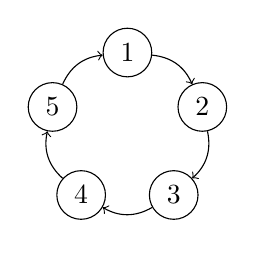
\begin{tikzpicture}[->]
                \foreach \i [count=\j from 1] in {90,18,...,-198} \node[circle,draw] (\j) at (\i:1) {\j};
                \path (1) edge [bend left] node [below] {} (2);
                \path (2) edge [bend left] node [below] {} (3);
                \path (3) edge [bend left] node [below] {} (4);
                \path (4) edge [bend left] node [below] {} (5);
                \path (5) edge [bend left] node [below] {} (1);
            \end{tikzpicture}
        \end{figure}
    \end{minipage} \hfill
    \begin{minipage}{0.45\textwidth}
    In this case all the states communicate, since it is possible to go from one to any other with at most 5$<\infty$ steps. 
    \end{minipage}
\end{example}
Communicating states form an \enf{equivalence class}: the relation is reflective, symmetric and transitive. This can be proved using the Chapman-Kolmogorov equation (Eq. \ref{chapkolm}). $S$ can be split in two or more classes of communicating states, thus obtaining a \textbf{macroscopic description} of the chain dynamics.
\begin{example}\label{irr}
\[
    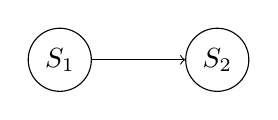
\begin{tikzpicture}[node distance=2cm]
        \node[circle,draw](2){$S_2$};
        \node[circle, draw](1)[left of=2]{$S_1$} edge[->] (2);
    \end{tikzpicture}
    \qquad S_1, S_2 \subset S
\]
In this case, once the chain leaves $S_1$ it can't go back. $S_2$ can be accessed by $S_1$ but not vice-versa. On the long run we can say that we should focus on $S_2$, since $S_1$ will be left for good sooner or later.
\end{example}

\subsubsection{Irreducibility
}
\begin{definition}
    A Markov chain with a single equivalence class generated by communicating states is said to be \enf{irreducible}.
\end{definition}
For instance, in the previous example the chain is not irreducible but once the chain leaves $S_1$ it becomes irreducible in $S_2$.\\
What about the main Markov processes?
\begin{itemize}
    \item The simple random walk is \sott{irreducible}: we can always go in every state;
    \item in branching processes, if $X_n=0$ then the process stops and $X_{n+1}=0$. This means that $\{1,2,\ldots\}$ are not accessible from 0 and the chain is therefore \sott{not irreducible};
    \item in Wright-Fisher process with no mutations we face a similar situation: $X_n=0\implies X_{n+1}=0 $ and $X_n=N\implies X_{n+1}=N $: $\{1,\ldots,N-1\}$ are not accessible from $\{0,N\}$ and the chain is therefore \sott{not irreducible}. The introduction of mutations, though, would make it irreducible.
\end{itemize}

\subsubsection{Periodicity}
\begin{definition}
    We define the \enf{period} $d(i)$ of $i\in S$ the greatest common divisor of all $n\geqslant 1$ such that $p_{ii}^{(n)}>0$. If $p_{ii}^{(n)}>0$ for all sufficiently large $n$ (or if $d(i)=1$) we say that $i$ is \enf{aperiodic}.
\end{definition}
\begin{example}
     \begin{minipage}{0.5\textwidth}
        \begin{figure}[H]
            \centering
            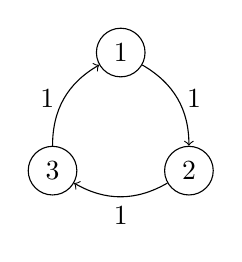
\begin{tikzpicture}[->,node distance=2cm]
                \foreach \i [count=\j from 1] in {90,-30,-150} \node[circle,draw] (\j) at (\i:1) {\j};
                \path (1) edge [bend left] node [right] {1} (2);
                \path (2) edge [bend left] node [below] {1} (3);
                \path (3) edge [bend left] node [left] {1} (1);
            \end{tikzpicture}
        \end{figure}
    \end{minipage} \hfill
    \begin{minipage}{0.45\textwidth}
        $\forall i=1,2,3:$\medskip \\
        $p_{ii}^{(3n)}=1\qquad \forall n+1$\\
        $p_{ii}^{(3n+1)}=0\qquad \forall n\geqslant 1$\\
        $p_{ii}^{(3n+2)}=0\qquad \forall n\geqslant 1$\\
        $d(i)=3 \qquad i\in S$
    \end{minipage}
\end{example}
Periodicity is a \enf{class property}: if $i,j$ communicate then they have the same period. This means that the period of the communication class $S_1$ is enough to study the period of a single $i\in S_1$.
\begin{example}
    The simple random walk is irreducible: $S = \mathbb{Z}$ is a single communicating class. For $i>0$:
    \[
    p_{00}^{(2n)}>0 \qquad p_{00}^{(2n+1)}=0 \qquad n \geqslant 0
    \]
    so the period is 2.
\end{example}

\begin{proposition}
    If $X$ is irreducible and $p_{ii}>0$ for some $i \in S$ then $X$ is aperiodic.
\end{proposition}
\begin{example}
     \begin{minipage}{0.5\textwidth}
        \begin{figure}[H]
            \centering
            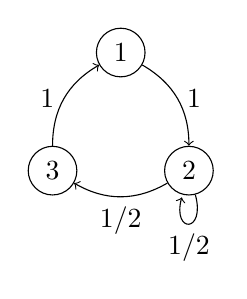
\begin{tikzpicture}[->,node distance=2cm]
                \foreach \i [count=\j from 1] in {90,-30,-150} \node[circle,draw] (\j) at (\i:1) {\j};
                \path (1) edge [bend left] node [right] {1} (2);
                \path (2) edge [bend left] node [below] {1/2} (3);
                \path (3) edge [bend left] node [left] {1} (1);
                \path (2) edge [loop below] node [below] {1/2} (2);
            \end{tikzpicture}
        \end{figure}
    \end{minipage} \hfill
    \begin{minipage}{0.45\textwidth}
        The chain is aperiodic: I can get from 3 back again to 3 in 3 steps of in 4,5,6,$\ldots$ if I cycle in 2.
        \[p_{33}^{(n)}>0\qquad n\geqslant 3.\]
        The greatest common denominator is 1: $d(3)=1$
    \end{minipage}
\end{example}
We can exploit this property: if $P$ is periodic, define
\[
P'=\varepsilon P+(1-\varepsilon)I,\hspace{2cm} \varepsilon\in(0,1)
\]
This is called the "\sott{lazy chain}" because the chain is not going to move from its state in $n$ with probability $\varepsilon$ and $P'$ is aperiodic. We will see that this modification essentially does not alter the distributional properties of the chain. 
\subsubsection{Recurrence}
Recall now the first visit to $i$
\[
T_i=\inf\{n\geqslant 1: X_n=i\}
\]

\begin{definition}
    A state $i$ is said do be \enf{recurrent} if \[\prob(T_i<\infty|X_0=i)=1\],  or equivalently \[\prob(T_i<\infty \quad\text{for some}\quad n|X_0=i)=1\] which means that the return time is finite almost surely. The state $i$ is otherwise said to be \enf{transient}.
\end{definition}
A transient $i$ is such that \[\prob(T_i<\infty|X_0=i)<1.\]It is worth noting that a transient state still has a positive probability of coming back on $\infty$.

\begin{proposition}
    Let $p_{ii}^{(n)}$ be the return probability to $i$ in $n$ steps. Then $i \in S$ is recurrent if and only if \[\sum_{n\geqslant 1} p_{ii}^{(n)}=\infty \] and it is transient otherwise.
\end{proposition}
Let $I_n=\mathbbm{1}(X_n=i)$:
\begin{align*}
    \sum_{n\geqslant 1} p_{ii}^{(n)}&=\sum_{n\geqslant 1} \prob(X_n|X_0=i)\\
    &=\lim_{N \to \infty}\sum_{n=1}^N\ev{I_n|X_0=i}\\
    &=\lim_{N \to \infty}\ev{\underbrace{\sum_{n=1}^NI_n}_{\mathclap{f_N}}|X_0=i}\\
    &=\ev{\sum_{n=1}^{\infty}I_n|X_0=i}\\
    &\text{\footnotesize(by monotone convergence theorem)}
\end{align*}
So $i$ is recurrent if in expectation it is visited $\infty$ many times over the whole time horizon. \\
We can define \[G:=\sum_{n\geqslant 0}p^n\] which is sometimes called \sott{potential matrix}.

\begin{proposition}
    A state $i$ is visited almost surely:
    \begin{itemize}
        \item infinitely often if recurrent;
        \item finitely often if transient
    \end{itemize}
\end{proposition}
Intuition: $T_i^{(1)}$ is the first passage time to $i$. If $i$ is recurrent then by definition
\[
\prob(T_i^{(1)}<\infty|X_0=i)=1.
\]
Since $X_{T_i^{(1)}}=i$, from the strong Markov property we get: \[X'=X_{T_i^{(1)}+n}\sim Markov(\delta_i,P)\]
so $X_{T_i^{(2)}}$ for $X$ is the first passage time for $X'$, which implies 
\[T_i^{(1)}\stackrel{d}{=}T_i^{(2)} \implies \prob(T_i^{(2)}<\infty|X_{T_i^{(1)}}=i)=1.\]
So over an infinite time horizon we have infinitely many visits with probability 1.

Recurrence is a class property, so if a chain is irreducible it is enough to check one state. If we checked that $i$ is recurrent all states that communicate with $i$ will be visited infinitely many times.

\begin{proposition}
    The simple random walk on $\mathbb{Z}$ is recurrent if and only if $p=\frac{1}{2}$, that is if the walk is symmetric. 
\end{proposition}

    \begin{proof2}
        To check that the chain is irreducible, it is enough to check that $i=0$ is irreducible:
        \[p_{00}^{(2n)}>0 \hspace{2cm}  p_{00}^{(2n+1)}=0 \qquad n\geqslant 1\] so it is enough to check the even number of steps:
        \begin{center}
            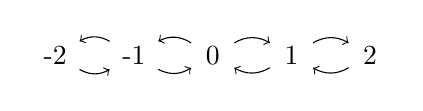
\begin{tikzpicture}[->]
                \node [circle] (zero) {0};
                \node [circle] (one) [right of=zero] {1};
                \node [circle] (two) [right of=one] {2};
                \node [circle] (mone) [left of=zero] {-1};
                \node [circle] (mtwo) [left of=mone] {-2};
                \path (zero) edge [bend left] node [right] {} (one);
                \path (one) edge [bend left] node [right] {} (two);
                \path (zero) edge [bend right] node [right] {} (mone);
                \path (mone) edge [bend right] node [right] {} (mtwo);
                \path (mtwo) edge [bend right] node [right] {} (mone);
                \path (mone) edge [bend right] node [right] {} (zero);
                \path (two) edge [bend left] node [right] {} (one);
                \path (one) edge [bend left] node [right] {} (zero);
            \end{tikzpicture}
        \end{center}
        I sample right and left steps $n$ times each:
        \[p_{00}^{(2n)}=\binom{2n}{n}p^n(1-p)^n\]
        Verify using Stirling's approximation that
        \[n!\approx \text{const}\times n^{n+\frac{1}{2}}e^{-n}\implies p_{00}^{(2n)}\approx \frac{[4p(1-p)]^n}{\sqrt{n}}\]
        so
        \[
            \sum_{n\geqslant 0}p_{00}^{(n)}\approx  \sum_{n\geqslant 0}\frac{[4p(1-p)]^n}{\sqrt{n}}
            \]
            \[
            \rightarrow\begin{cases}
                <\infty &4p(1-p)<1=p(1-p)<\frac{1}{4}\; \text{which means}\;p\neq \frac{1}{2}\\
                =\infty &p=\frac{1}{2}
            \end{cases}
            \]
        which means that the series is infinite when $p=1/2$.
    \end{proof2}
What about a random walk on $\Z^d$? 
\[
d=2,\; i,j\in\Z^2 \qquad p_{ij}=\begin{cases}
    \frac{1}{4} &\text{if}\quad|i_1-j_1|+|i_2-j_2|\\
    0 &\text{else}.
\end{cases}
\]
 \begin{minipage}{0.5\textwidth}
        \begin{tikzpicture}[
            >=stealth', axis/.style={<->},
            point/.style={circle, inner sep=0pt, fill, minimum size=4pt, label=#1},
            scale=.75]
        \draw[axis] (0,-3) -- (0,3) node[above right]{$y$};
        \draw[axis] (-3,0) -- (3,0) node[below right]{$x$};
        \draw[dashed,RedViolet] (0,0) -- (3,3);
        \draw[dashed,RedViolet] (1.5,1.5) -- (3,0);
        \draw[dashed,RedViolet] (0,0) -- (3,-3);
        \draw[dashed,RedViolet] (1.5,-1.5) -- (3,0);
        \coordinate (A) at (1.5,1.5);
        \coordinate (B) at (0,0);
        \draw [|-|]([yshift=0.1cm,xshift=-0.1cm]A) -- ([yshift=0.1cm,xshift=-0.1cm]B)node [black,midway,sloped,above]{$\frac{1}{\sqrt{2}}$};
        \end{tikzpicture}
    \end{minipage} \hfill
    \begin{minipage}{0.45\textwidth}
    The random walk on $\Z^2$ can be seen as 2 independent random walk on the diagonals of the cartesian plane.
    \end{minipage}
\begin{align*}
    &p_{(0,0),(0,0)}^{(2n+1)}=0\\
    &p_{(0,0),(0,0)}^{(2n)}=\Biggl[\underbrace{\binom{2n}{n}\biggl(\frac{1}{2}\biggr)^n\biggl(\frac{1}{2}\biggr)^n}_{\mathclap{\approx \frac{1}{\sqrt{n}}}}\Biggr]^2\\
    &\sum_{n \geqslant 0}p_{(0,0),(0,0)}^{(n)}=\infty\implies\text{the chain is recurrent.}
\end{align*}
Consider now a symmetric random walk on $\Z^3$:
\[
    \sum_{n \geqslant 0}p_{(0,0,0),(0,0,0)}^{(n)}=\Biggl[\underbrace{\binom{2n}{n}\biggl(\frac{1}{2}\biggr)^n\biggl(\frac{1}{2}\biggr)^n}_{\mathclap{\approx \frac{1}{\sqrt{n}}}}\Biggr]^3\approx\frac{1}{n^{\frac{3}{2}}}
\]
This is a convergent series, which means that from 3 dimensions onward the random walk \textit{is transient}.

In the transient case we have:
\[
\sum_{n\geqslant 1}p_{ii}^{(n)}<\infty\implies p_{ii}^{(n)}\xrightarrow[n\rightarrow\infty]{}0
\]
It can be proved that $\forall j \in S$, $p_{ii}^{(n)}\xrightarrow[n\rightarrow\infty]{}0$. In the recurrent case, where we have $\sum p_{ii}^{(n)}=\infty$:
\begin{itemize}
    \item $p_{ii}^{(n)}\rightarrow c>0$, which causes the \textit{divergence} of the series;
    \item  $p_{ii}^{(n)}\rightarrow 0$ but slowly, not faster than $\frac{1}{n}$, causing divergence in this case as well.
\end{itemize}
But is this dichotomy useful? define
\[m_i=\ev{T_i|X_0=i}\] as the \enf{mean return time to} $\enf{i}$. If $i$ is transient, then \[\prob(T_i<\infty|X_0=i)<1\implies\prob(T_i=\infty|X_0=i)>0\implies m_i=\infty\].

\begin{definition}
    A recurrent state $i$ is called:
    \begin{itemize}
        \item \enf{positive} if $m_i<\infty$
        \item \enf{null} if $m_i=\infty$
    \end{itemize}
    and these are \textit{class properties}.
\end{definition}
Later we will show that a \sott{null recurrent} state $i$ is such that $p_{ji}^{(n)}\rightarrow 0$ $\forall j\in S$, so transient and null/positive recurrence can be understood in terms of the \sott{tail of the distribution} of the return times:
\begin{itemize}[-]
    \item positive probability at $\infty$ $\rightarrow$ transience
    \item probability mass is on $\N$ but it is not integrable ("heavy tailed") $\rightarrow$ null recurrence
    \item probability mass is on $\N$ and it is integrable $\rightarrow$ positive recurrence
\end{itemize}
\begin{example}
    The symmetric random walk on $\Z$ and $\Z^2$ are the only recurrent cases:
    \[p_{00}^{(2n)}\propto\frac{1}{\sqrt{n}} \hspace{2.7cm} p_{(0,0),(0,0)}^{2n}\propto\frac{1}{n} \]
    Both tend to 0 as $n$ tends to $\infty$, which means that both the states are null recurrent.
\end{example}
We are now interested in establishing how a chain can be classified as positive recurrent.

\begin{proposition}
    On a finite $S$, an irreducible chain is positive recurrent.
\end{proposition}
    \begin{proof2}
        \[S=\{0,\ldots,N\}\]
        \[\forall n\geqslant1:\qquad\sum_{j=0}^N p_{ij}^{(n)}=1. \]
        This means that we cannot have $p_{ji}^{(n)}\rightarrow 0$ $\forall j\in S$. So there exist a state $i \in S$ that is both positive and irreducible and therefore $X$ must be positive
    \end{proof2} 
\begin{example}
    Consider a Wright-Fisher chain with $S={0,\ldots,N}$. It has:
    \begin{align*}
        X_n=0 &\implies X_{n+1}=0\\
        X_n= &\implies X_{n+1}
    \end{align*}
    so $S$ is finite but $X$ is not irreducible.
    \[
    \begin{tikzpicture}[->,>=stealth',shorten >=2pt, line width=0.5pt, node distance=1.5cm]
        \node[circle, draw](1){$S_1$};
        \node[circle, draw](2)[above right of=1]{$S_2$};
        \node[circle, draw](3)[below right of=1]{$S_3$};
        \path (1) edge (2);
        \path (1) edge (3);
        \node[text width=4cm] [below of=3] {Case without off mutations};
    \end{tikzpicture}\hspace{3cm}
     \begin{tikzpicture}[<->,>=stealth',shorten >=2pt, line width=0.5pt, node distance=1.5cm]
        \node[circle, draw](1){$S_1$};
        \node[circle, draw](2)[above right of=1]{$S_2$};
        \node[circle, draw](3)[below right of=1]{$S_3$};
        \path (1) edge (2);
        \path (1) edge (3);
        \node[text width=4cm] [below of=3] {Case with odd mutations;};
    \end{tikzpicture}
    \]
    More generally, the task can be difficult. Often, so-called \textit{Lypaunov methods} are useful as a sufficient conidition.
\end{example}

\begin{proposition}
    Let $P$ be irreducible and let $h:S\rightarrow\R$ be such that $h(i)\geqslant0 \;\forall i \in S$ and:
    \begin{itemize}
        \item $\sum_{k\in S} p_{ik} \cdot h(k)<\infty\qquad\forall i \in S_0$
        \item $\sum_{k\in S} p_{ik} \cdot h(k)\leqslant h(i)\cdot \varepsilon\qquad\forall i \notin S_0$
    \end{itemize}
    for a finite set $S_0 \subset S$ and some $\varepsilon>0$. Then $P$ is positive recurrent.
\end{proposition}
The role of $h(\cdot)$ is similar to the one of Lyopunov function used for the stability of ODEs. Here
\[\sum_{k} p_{ik} \cdot h(k)-\ev{h(x_{n+1}|X_n=1)}\]
The second condition says that $h(\cdot)$ decreases in expectation outside $S_0$: $S_0$ is \enf{attractive}.
\begin{example}
    $S+\Z_+, \qquad h(i)=i$. The condition requires
    \[\ev{X_{n+1}-X_{n}|X_n=1}<0, \qquad i>i_0\]
    so the chain is atracted to the set $\{i:i\leqslant i_0\}$, giving stochastic stability.
\end{example}
\subsubsection{Stationarity}
Note:
\begin{align*}
    \prob(X_n=j) &= \overbrace{\sum_{i\in S}\prob(X_0=i)\prob(X_n=j|P_0=i) }^{\mathclap{\text{disintegrating the joint}}}\\
    &=\sum_{i\in S}\lambda_i p_{ij}^{(n)}=\left(\lambda P^n\right)_j
\end{align*}
$\left(\lambda P^n\right)_j$ can be seen as the marginal distribution of $X$ at time $n$: in other words
\[X_0\sim \lambda\implies X_n\sim\lambda P^n\]

\begin{definition}
    A non negative (row) vector $\pi=(\pi_i, i\in S)$ is said to be an \enf{invariant measure} for $P$ if $\pi P=\pi$, called \enf{global balance equation}. Namely:
    \[\sum_{i \in S} \pi_i p_{oj}=\pi_j \]
    i.e. marginalizing out the initial state with respect to $\pi$, the marginal measure after one step is preserved:
    \[
    X_0 \sim \pi \implies X_i \sim \pi P = \pi
    \]
\end{definition}
Furthermore,
\[
\pi P^2=\underbrace{\pi P}_{\pi}=\pi P= \pi
\]
Iterativity yields that $\pi P^n=\pi$, therefore
\[
X_0\sim \pi \implies X_n\sim\pi \qquad \forall n \geqslant 0
\]
We have extended the one-step invariance to the $n$-step invariance. If we can normalize $\pi$:
\[
\Tilde{\pi}_i=\frac{\pi_i}{\sum_{j\in S}\pi_j}\Tilde{\pi}\]
and we call $\Tilde{\pi}$ \enf{stationary distribution}.
\begin{example}
        \begin{figure}[H]
            \centering
            \begin{tikzpicture}[->,>=stealth',shorten >=2pt, line width=0.5pt, node distance=2cm]
                \node [circle, draw] (zero) {0};
                \node [circle, draw] (one) [right of=zero] {1};
                \path (zero) edge [bend left] node [above] {$\alpha$} (one);
                \path (zero) edge [loop left] node [left] {$1-\alpha$} (zero);
                \path (one) edge [loop right] node [right] {$1-\beta$} (zero);
                \path (one) edge [bend left] node [below] {$\beta$} (zero);
            \end{tikzpicture}
        \end{figure}
 with $\pi=(\pi_0,\pi_1)$, $\pi_i>0$.
    We need to try and solve the global balance equation:
    \[
    \pi P=\begin{bmatrix}
        \pi_0 & \pi_1
        \end{bmatrix}\begin{bmatrix}
            1-\alpha & \alpha \\
            \beta & 1-\beta
        \end{bmatrix}=\begin{bmatrix}
            \pi_0(1-\alpha)+\pi_1\beta & \pi_0\alpha+\pi_1(1-\beta)
        \end{bmatrix}.
    \]
    Impose $\pi P=\pi=(\pi_0, \pi_1)$:
    \[
    \pi_0(1-\alpha)+\pi_1\beta=\pi_0 \implies \pi_0=\pi_1\frac{\beta}{\alpha}.
    \]
    Substituting,
    \[
    \pi_1\frac{\beta}{\cancel{\alpha}}\cancel{\alpha}+\pi_1\beta=\pi_1 \implies \pi_1=\pi_1 \quad\tikz\fill[scale=0.4](0,.35) -- (.25,0) -- (1,.7) -- (.25,.15) -- cycle;
    \]
    with normalization we get
    \begin{align*}
        \pi_0+\pi_1=1&\longrightarrow{}\pi_1\frac{\beta}{\alpha}+\pi_1=1\\
        &\longrightarrow\pi_1=\frac{\beta}{\alpha+\beta},\quad\pi_0=\frac{\alpha}{\alpha+\beta}.
    \end{align*}
\end{example}
\begin{example}
    If $P$ is stationary with respect to $\pi$ then its "lazy" version \[P'=\varepsilon P+(1-\varepsilon)I,\quad\varepsilon\in[0,1]\]is still stationary.
\end{example}
\begin{example}
    Consider the random walk on $\Z$. The global balance equation is:
    \begin{align*}
        \sum_{i \in S} \pi_i p_{ij}&=\pi_{j-1}p_{j-1,j}+\pi_{j+1}p_{j+1,j}\\
        &=\pi_{j-1}p+\pi_{j+1}(1-p)\stackrel{?}{=}\pi_j
    \end{align*}
    Set $\pi_i=c\geqslant0$:
    \[cp+c(1-p)=c\]
    So:\begin{itemize}
        \item the uniform measure on $\Z$ is invariant;
        \item the invariant measures are not necessarily unique;
        \item $p\neq\frac{1}{2}$ is the transient case, $p=\frac{1}{2}$ is the recurrent case.
    \end{itemize}
    So there exists an invariant measure that doesn't imply recurrence.
    \[
    \sum_{i\in\Z}\pi_i=\begin{cases}
        \infty &c>0\\
        0 &c=0
    \end{cases}
    \]
    We cannot normalize in this case ($\pi$ is only $\sigma$-finite, not finite) so we have invariant measures but we don't have any stationary distribution: the chain is \sott{non stationary}.
\end{example}
\begin{exercise}
    Find the stationary distribution for $RW(p,1-p)$ and $p_{00}=1-p$ under correct restrictions on $p$.
\end{exercise}
\begin{exercise}
    Do the same for $B\&D(p,1-p)$ and $p_{00}=1-p$ under the correct restrictions on $p$.
\end{exercise}
\begin{exercise}
    Show that in $B\&D(p,1-p)$:
    \begin{align*}
        p_i&=\frac{b}{b+i},\quad b>0\\
        \implies\pi_i&=\frac{b+i}{2b}\sim Poiss(i,b)
    \end{align*}
    (called \sott{size-biased Poisson}).
\end{exercise}
We are interested in conditions that provide stationarity:

\begin{proposition}
    If for some $i\in S$ \[
    p_{ij}^{(n)}\xrightarrow[n\rightarrow\infty]{}\pi_j\implies\pi\text{ is invariant.}
    \]
\end{proposition}
    \begin{proof2}
        \[S=\{0,\ldots,N\}\]
        \[\forall n\geqslant1:\qquad\sum_{j=0}^N p_{ij}^{(n)}=1. \]
        This means that we cannot have $p_{ji}^{(n)}\rightarrow 0$ $\forall j\in S$. So there exist a state $i \in S$ that is both positive and irreducible and therefore $X$ must be positive
    \end{proof2} 
\begin{example}
    Consider the random walk on $\Z$:
    \[p_{ij}^{(n)}\rightarrow0\implies\pi=(\pi_i,i\in\Z)\quad\pi_i=0\]
    Which is invariant, as found above, with $c=0$.
\end{example}
\begin{example}
    \[
    P=\begin{bmatrix}
            1-\alpha & \alpha \\
            \beta & 1-\beta
        \end{bmatrix}\qquad\alpha,\beta\neq 1
    \]
    \begin{align*}
        p_{00}^{(n+1)}&\equalexpl{\text{C.K.}}\hspace{1em}\sum_{k\in S}p_{0k}^{(n)}p_{k0}=p_{00}^{(n)}\underbrace{(1-\alpha}_{p_{00}}+\underbrace{pp{01}^{(n)}}_{1-p_{00}^{(n)}}\underbrace{\beta}_{p_{10}}\\
        p_{00}^{(n+1)}&=\ldots=\beta+p_{00}^{(n)}(1-\alpha-\beta)
    \end{align*}
    The recurrence equation brings to solution:
    \[p_{00}^{(n)}=\frac{\beta}{\alpha+\beta}+(1-\alpha-\beta)^n\frac{\alpha}{\alpha+\beta}\rightarrow\frac{\beta}{\alpha+\beta}\]
    as found earlier.
\end{example}
In general we do not want to assume that $P^n$ converges.
\begin{theorem}
     An irreducible Markov Chain has invariant distribution $\pi$ if and only if it is positive recurrent, in which case $\pi$ is unique and 
        \begin{equation*}
            \pi_i = \frac{1}{m_i}
        \end{equation*}
        where 
        \begin{equation*}
            m_i = \ev{T_i | X_0 = i}
        \end{equation*}
        is the \textbf{expected return time}. 
\end{theorem}
\begin{example}
    Considering $P=I$, we found out that the invariant distribution is not unique. This is a contradiction, due to the fact that irreducibility is violated.
\end{example}
\begin{example}
    Consider a random walk on $\mathbb{Z}$ for $p \in (0,1)$ which is transient and null recurrent: This implies that $m_i = \infty$. Indeed $\pi_i = \frac{1}{m_i} = 0$ is invariant for the random walk. 
\end{example}
\begin{example}
    Consider a 2-state chain with
    \begin{equation*}
        (\pi_0, \pi_1) = (\frac{\beta}{\alpha + \beta}, \frac{\alpha}{\alpha + \beta}).
    \end{equation*}
    If we interpret the statement literally, then\[(m_0,m_1)= (\frac{\alpha +\beta}{\beta}, \frac{\alpha + \beta}{\alpha})\]
    Let's choose, for example,  $\alpha = 0.5$ and $\beta = 1$:\[   
    \begin{tikzpicture}[->,>=stealth',shorten >=2pt, line width=0.5pt, node distance=2cm]
        \node [circle, draw] (zero) {0};
        \node [circle, draw] (one) [right of=zero] {1};
        \path (zero) edge [bend left] node [above] {$\frac{1}{2}$} (one);
        \path (zero) edge [loop left] node [left] {$\frac{1}{2}$} (zero);
        \path (one) edge [bend left] node [below] {$1$} (zero);
    \end{tikzpicture}\]
    with $m_0=\frac{3}{2}$ and $m_1=3$
    We can double check:
    \begin{itemize}
        \item Return to 0: $\begin{cases}
            1 &\text{ with probability } \frac{1}{2}\\
            2 &\text{ with probability } \frac{1}{2}\\
        \end{cases}$ $\implies 1 \cdot \frac{1}{2} + 2 \cdot \frac{1}{2} = \frac{3}{2} = m_0$
        \item Return to 1: $\begin{cases}
            2 &\text{ with probability } \frac{1}{2}\\
            3 &\text{ with probability } \frac{1}{2^2}\\
            \vdots \\
            (1+k) &\text{ with probability } \frac{1}{2^k}\\
            \vdots\\
        \end{cases}$
        so\[m_1 = \sum_{k \geq 1} (1+k) \frac{1}{2^k} = \ldots = \sum_{k \geq 1} \frac{1}{2^k} + \sum_{k \geq 1} \frac{k}{2^k} = 1+2 = 3.\]
    \end{itemize}
\end{example}
\begin{definition}
    An irreducible Markov chain is said to be \enf{reversible  with respect to $\pi$} if 
\[
            \pi_i p_{ij} = \pi_j p_{ji} \hspace{1 cm} \forall i,j \in S  \hspace{1 cm} \]
        which is called \enf{detailed balance equation}.
\end{definition}\begin{proposition}
    If $P$ and $\pi$ are in detailed balance (that is, they satisfy the detailed balance equation, then $\pi$ is invariant for $P$.
\end{proposition}
    
    \begin{proof2}
        Integrate both sides of the equation with respect to $i$:
        \begin{align*}
            \sum_i\pi_ip_{ij}&= \sum_i\pi_jp_{ij}\\
            &=\pi_j\underbrace{\sum_ip_{ij}}_{=1}=\pi_j.
        \end{align*}
    \end{proof2}
Detailed balance is a sort of \sott{local criterion} on the chain propensity to go from $i\rightarrow j$ and $j \rightarrow i$, while the global balance is a \sott{global criterion} on the chain propensity to go from $i\rightarrow j$ and $j \rightarrow i$.
\begin{example}
     \begin{minipage}{0.5\textwidth}
     \center
        \begin{tikzpicture}[->,>=stealth',node distance=2cm]
                \foreach \i [count=\j from 0] in {150,30,-90} 
                \node[circle,draw] (\j) at (\i:1.3) {\j};
                \path (0) edge [bend left] node [above] {\footnotesize 2/3} (1);
                \path (1) edge [bend left] node [below right] {\footnotesize 2/3} (2);
                \path (2) edge [bend left] node [below left] {\footnotesize 2/3} (0);
                \path (1) edge [bend left] node [above] {\footnotesize 1/3} (0);
                \path (2) edge [bend left] node [right] {\footnotesize 1/3} (1);
                \path (0) edge [bend left] node [left] {\footnotesize 1/3} (2);
        \end{tikzpicture}
    \end{minipage} \hfill
    \begin{minipage}{0.45\textwidth}
    Check first that the uniform distribution is invariant: \[\pi = (\frac{1}{3}, \frac{1}{3}, \frac{1}{3}).\] 
    Nevertheless, 
    \[
        \pi_0 p_{01} = \frac{1}{3} \frac{2}{3} \neq \frac{1}{3}\frac{1}{3} = \pi_1 p_{10}
    \]
    \end{minipage}
\end{example}
\begin{example}
    Consider a Birth and Death process of parameters $(p,1-p)$ with 
    \begin{equation*}
        p_{00} = 1-p
    \end{equation*}
    The detailed balance equation is
    \begin{equation*}
        \pi_i p_{ij} = \pi_j p_{ji}   \hspace{1 cm} \forall i,j
    \end{equation*}
    Take $j=i+1$: we get
    \begin{align*}
        \pi_i p_{i,i+1} &= \pi_{i+1} p_{i+1,i}  \hspace{1 cm} q:=1-p \\
        \pi_i p &= \pi_{i+1} q\\
        i = 0 &\implies \pi_1 = \pi_0 \frac{p}{q}\\
        i = 1 &\implies \pi_2 = \pi_1 \frac{p}{q} = \pi_0 \Big(\frac{p}{q}\Big)^2 \\
        &\implies \pi_k = \pi_0 \Big(\frac{p}{q}\Big)^k
    \end{align*}
    So, $\pi_k$ is proportional to $\rho^k$, where $\rho = \frac{p}{q}$. \\
    We now integrate $\pi_k$:
    \begin{equation*}
        \sum_{k \geq 0} \pi_k < \infty \iff p < \frac{1}{2} \hspace{0.5 cm} (\rho < 1) + \ldots
    \end{equation*}
    which implies that 
    \begin{equation*}
        \Tilde{\pi} = \frac{\pi_k}{\sum_j \pi_j} \sim \text{Geom}(\rho).
    \end{equation*}
    So, using detailed balance equations, we get a result faster than what we would obtain through global balance equations.
\end{example}
Let 
\begin{equation*}
    <x,y>:= \sum_{i \in S} x_i y_i \pi_i.
\end{equation*}
\begin{definition}
    We define 
        \begin{equation*}
            \ell_2(\pi) := \{x \in \mathbb{R}^S: <x,x> < \infty\}.
        \end{equation*}
        A matrix $P$ is \enf{self-adjoint with respect to} $\pi$ if 
        \begin{equation*}
            <Px,y> = <x, Py>, \hspace{1 cm} x,y \in \ell_2(\pi).
        \end{equation*}
\end{definition}\begin{proposition}
     Markov chain with transition matrix $P$ is reversible with respect to $\pi$ if and only if $P$ is self-adjoint with respect to $\pi$.
\end{proposition}
It can be proved that if $P$ is reversible with respect to $\pi$, then the \enf{time reversal}
        \begin{equation*}
            Y_n := X_{N-n}, \hspace{1 cm} 0 \leqslant n \leqslant N
        \end{equation*}
        has the same distribution as $X$ if both are started in equilibrium.
\subsubsection{Convergence}
We can interpret time reversal as the possibility of reversing the sense of time. If the chain $X$ starts from an arbitrary initial distribution, not necessarily at equilibrium, is it going to converge to the stationary distribution?
\begin{equation*}
    \lambda P^n \xrightarrow[\text{?}]{n \rightarrow \infty} \pi
\end{equation*}
The notion of convergence convergence has to be made more precise.
\begin{example}
    Consider the matrix $P$:\\
    \begin{minipage}{0.5\textwidth}
     \center
        \[P=\begin{bmatrix}
        0 & 1 \\
        1 & 0 \\
    \end{bmatrix}\]
    \end{minipage} \hfill
    \begin{minipage}{0.45\textwidth}
    \begin{figure}[H]
            \centering
            \begin{tikzpicture}[->,>=stealth',shorten >=2pt, line width=0.5pt, node distance=2cm]
                \node [circle, draw] (zero) {0};
                \node [circle, draw] (one) [right of=zero] {1};
                \path (zero) edge [bend left] node [above] {} (one);
                \path (one) edge [bend left] node [below] {} (zero);
            \end{tikzpicture}
        \end{figure}
    \end{minipage}
    The chain is 
    \begin{itemize}
        \item [-] irreducible 
        \item [-] positive-recurrent (the mean return time, which is the only return time, equals $2$)
        \item [-] The stationary distribution
        \begin{equation*}
            \pi = (\frac{1}{2}, \frac{1}{2}) 
        \end{equation*}
        is invariant \checkmark
        \end{itemize}
     But, 
    \begin{itemize}
        \item [-] $P^{2n+1} = P, \;P^{2n} = I$, so $p_{ij}^{(n)} \not\rightarrow \pi_j$. Previously, we assumed convergence and  said that a limiting distribution is invariant
        \item [-] $\lambda P^{2n} = \lambda \hspace{1 cm} \lambda P^{2n+1}=1-\lambda$
    \end{itemize}
    Why? The periodicity is \sott{preventing the chain to converge}. Periodicity prevents convergence by making the dependence on the initial state too strong: if the chain starts from 0 the all even steps will bring to 0 and all odd steps will bring to 1.
\end{example}
\begin{definition}
    An irreducible, aperiodic, positive recurrent chain is called \enf{ergodic}.
\end{definition}
Under these assumptions, we want to show that an ergodic chain converges to equilibrium from any initial distribution. To do so, we are going to use \sott{\textit{coupling}}. Consider
\begin{itemize}
    \item $\pi$ invariant for $P$
    \item $X \sim$ Markov $(\lambda, P)$. $\lambda$ is arbitrary and the so distributed $X$ is the chain of interest.
    \item $Y \sim$ Markov $(\pi, P)$ is an auxiliary chain
    \[\implies Y_n \sim \pi, \forall n \geq 0\]
    \item Assume $X$ and $Y$ meet in finite time.
\end{itemize}
\begin{figure}[H]
    \centering
    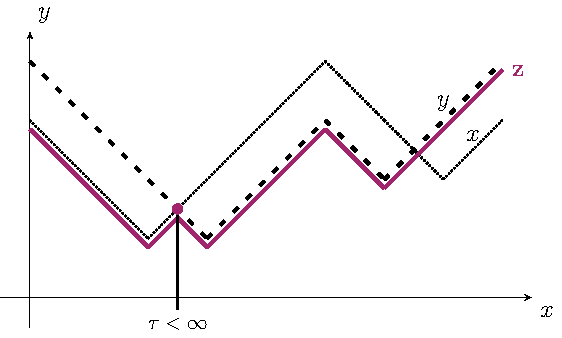
\includegraphics{../standalones/pdfs/coupling}
\end{figure}
We obtain a new chain $Z_n$ so defined:
\[
Z_n = 
\begin{cases}
    X_n & n<\tau \\
    Y_n & n \geq \tau \\
\end{cases}
\]
Now, \underline{if} we show that $Z \sim$ Markov $(\lambda, P)$ (reaching quote $2$ assumptions, together with meeting in finite time), then 
\[
    X \stackrel{d}= Z \qquad\text{and}\qquad
    Z_n \sim \pi \hspace{0.5 cm} \forall n \geq \tau\]
which would imply that 
\begin{equation*}
    X_0 \sim \lambda, X_n \xrightarrow{n \rightarrow \infty} \pi 
\end{equation*}
\begin{definition}
    Two Markov chains $Z$ and $Y$ on $S$ are said to \enf{couple} if there exists an almost surely finite stopping time $\tau$, called \enf{coupling time}, such that 
        \begin{equation*}
            Z_n = Y_n \hspace{1 cm} \forall n \geq \tau
        \end{equation*}
\end{definition}
This relates to the \enf{total variation distance} between the marginals:
\begin{equation*}
    V \sim \lambda,\; W \sim \mu \text{ on } S
\end{equation*}
The total variation distance is 
\begin{align*}
    d_{TV}(\lambda,\mu) &= \sup_{A \subset S} |\mathbb{P}(V \in A) - \mathbb{P}(W \in A)| \\
    &= \frac{1}{2} \sum_{i \in S} |\lambda_i - \mu_i|
\end{align*}
\begin{proposition}
    \label{totvardist}
        Let $Z \sim$ Markov$(\lambda, P)$ and 
        let $Y \sim$ Markov$(\mu, P)$; \\
        assume that a coupling time exists. Then,
        \begin{equation*}
            d_{TV}(\lambda P^n, \mu P^n) \xrightarrow{n \rightarrow \infty} 0
        \end{equation*}
\end{proposition}

        \begin{proof2}
            Consider $A \subset S$ and 
        \begin{align*}
            \mathbb{P}(Z_n \in A) - \mathbb{P}(Y_n \in A) &= \mathbb{P}(Z_n \in A, n < \tau) + \mathbb{P}(Z_n \in A, n \geq \tau) +\\
            &- \mathbb{P}(Y_n \in A, n < \tau) - \mathbb{P}(Y_n \in A, n \geq \tau) \\
            &\stackrel{Z_n = Y_n, \forall n \geq \tau}= \mathbb{P}(Z_n \in A, n < \tau)- \underbrace{\mathbb{P}(Y_n \in A, n < \tau)}_{\geq 0} \\
            &\leq \mathbb{P}(\underbrace{Z_n \in A, n < \tau}_{\subset \{n < \tau\}})\\
            &\leq \mathbb{P}(n < \tau)
        \end{align*}
        Hence, by the arbitrarity of $A$,
        \begin{equation*}
            \sup_{A \subset S} |\mathbb{P}(Z_n \in A) - \mathbb{P}(Y_n \in A)| \leq \mathbb{P}(\tau > n)
        \end{equation*}
        but $\tau < \infty$ almost surely, so
        \begin{equation*}
            \mathbb{P}(\tau > n) \xrightarrow{n \rightarrow \infty} 0
        \end{equation*}
        \end{proof2}
So, we are sure that in a finite time they meet and hence $Z$ is going to have the stationary distribution $\pi$. Also, 
\begin{equation*}
    \exists \tau < \infty \implies d_{TV} \rightarrow 0
\end{equation*}
It is enough to show that such $\tau$ exists for ergodic chains. 
\begin{theorem}
     Let 
        \begin{itemize}
            \item $P$ be ergodic 
            \item $X \sim$ Markov$(\lambda, P)$ and $Y \sim $ Markov$(\mu, P)$ be independent 
        \end{itemize}
        Then, the stopping time 
        \begin{equation*}
            \tau = \inf\{n \geq 0: X_n = Y_n\}
        \end{equation*}
        is almost surely finite, and the chain
        \[
        Z_n =   
        \begin{cases}
            X_n & n<\tau \\
            Y_n & n \geq \tau \\
        \end{cases}
        \]
        is Markov$(\lambda, P)$.
\end{theorem}
So, this yields a coupling time between $Z \sim$ Markov$(\lambda, P)$ and $Y \sim$ Markov $(\mu, P)$, which implies that 
\begin{equation*}
    Z_n = Y_n \sim \mu P^n, \forall n \geq \tau
\end{equation*}
So, by the Proposition \ref{totvardist}, 
\begin{equation*}
    d_{TV}(\lambda P^n, \mu P^n) \xrightarrow{n \rightarrow \infty} 0
\end{equation*}
If we now let $\mu = \pi$, then $\mu P^n = \pi$ and hence 
\begin{equation*}
    d_{TV}(\lambda P^n, \pi) \rightarrow 0
\end{equation*}
\begin{remark}
        Imposing $\mu = \pi$ is not cheating since $\mu$ is auxiliary and we can equal it to what we need. The result is that all the marginals converge to the stationary. 
\end{remark}
Since $X \stackrel{d} = Z$, then
\begin{equation*}
    \mathbb{P}(X_n = j) \xrightarrow{n \rightarrow \infty} \pi_j, \hspace{1 cm} \text{ for every initial distribution } \lambda
\end{equation*}
If $\lambda = \delta_i$:
\begin{align*}
    d_{TV}(\lambda P^n, \pi) &= \frac{1}{2} \sum_{j \in S} |(\lambda P^n)_j - \pi_j| \\
    &= \frac{1}{2} \sum_{j \in S} |\sum_h \lambda_h p_{hj}^{(n)} - \pi_j| \\
    &= \frac{1}{2} \sum_{j \in S} |1 \cdot p_{ij}^{(n)}-\pi_j| \xrightarrow{n \rightarrow \infty} 0
\end{align*}
\begin{remark}
        In the first line, we take the supremum over a discrete space, so in the worst case we integrate the differences. 
\end{remark}
Hence, all the transition probabilities 
\begin{equation*}
    p_{ij}^{(n)} \xrightarrow{n \rightarrow \infty} \pi_j, \forall i \in S
\end{equation*}
converge to $\pi_j$ for every starting point (state) $i$.\\
In summary:
\begin{theorem}
    \label{th erg}
        Let $P$ be ergodic with invariant distribution $\pi$, and let $X \sim$ Markov$(\lambda, P)$. Then,
        \begin{equation*}
            d_{TV}(\lambda P^n, \pi) \xrightarrow{n \rightarrow \infty} 0
        \end{equation*}
        and
        \begin{equation*}
            p_{ij}^{(n)} \xrightarrow{n \rightarrow \infty} \pi_j, \hspace{1 cm} \forall i,j \in S. 
        \end{equation*}
\end{theorem}
\begin{remark}
        Ergodicity ensures that the two chains meet on the diagonal. $\lambda$ is orthogonal to $\mu$ and there exists $B \in S$ such that 
    \begin{align*}
        &\sum_{i \in B} \lambda_i = 1 \\
        &\sum_{i \in B^C} \mu_i = 1 \\
    \end{align*}
\end{remark}
\begin{example}
     Consider the matrix $P$:\\
    \begin{minipage}{0.5\textwidth}
     \center
        \[P=\begin{bmatrix}
        0 & 1 \\
        1 & 0 \\
    \end{bmatrix}\]
    \end{minipage} \hfill
    \begin{minipage}{0.45\textwidth}
    \begin{figure}[H]
            \centering
            \begin{tikzpicture}[->,>=stealth',shorten >=2pt, line width=0.5pt, node distance=2cm]
                \node [circle, draw] (zero) {0};
                \node [circle, draw] (one) [right of=zero] {1};
                \path (zero) edge [bend left] node [above] {} (one);
                \path (one) edge [bend left] node [below] {} (zero);
            \end{tikzpicture}
        \end{figure}
    \end{minipage}
    We know that \[
        \pi = (\frac{1}{2}, \frac{1}{2}) \qquad\text{and}\qquad P^{(2n)} = I, P^{(2n+1)} = P \]
    Consider also $X, Y$ as characterized in Theorem \ref{th erg}, with $\lambda = \delta_0, \mu = \pi$. This means that $X$ starts at $0$ with probability $1$:
    \begin{align*}
        X_0 &= 0 \text{ a.s.} \\
        Y_0 &=
        \begin{cases}
            0 &\text{ with probability } \frac{1}{2} \\
            1 &\text{ with probability } \frac{1}{2} \\
        \end{cases}
    \end{align*}
    So, either they meet at $n = 0$ or they never meet. 
\end{example}
It's useful to remind that are talking about almost sure meeting, not with probability $1$. Which factor breaks the conclusion of meeting almost surely? The chain is:
\begin{itemize}
    \item positive recurrent;
    \item irreducible;
    \item \sott{not} aperiodic.
\end{itemize}
\begin{theorem}
    \enf{Ergodic theorem}. Let $X\sim Markov(\lambda,P)$ be irreducible and let $m_i=\mathbb{E}\Bigl[T_i|X_0=i\Bigr]$. Then, almost surely,
        \[\frac{1}{N}\sum_{n=1}^N\mathbbm{1}(X_n=j)\xrightarrow[N\rightarrow\infty]{}\Pi_j=\frac{1}{m_j}.\]
        Moreover, if $P$ is positive recurrent with unique stationary distribution $\pi$ and $f:S\rightarrow\mathbb{R}$ with respect to $\pi$, then
        \[\frac{1}{N}\sum_{n=1}^Nf(X_n)\xrightarrow[N\rightarrow\infty]{}\sum_{j\in S}f(j)\Pi_j.\]
\end{theorem}
The quantity $\frac{1}{N}\sum_{n=1}^Nf(X_n)$ is the \textbf{ergodic average} and it is taken along the sample path of the chain. The right-hand side shows an object whose form recalls an expectation. \\
So, this is a way of relaxing the assumption of an i.i.d. sample. We are substituting it with the correlation associated to the Markovian structure, so that the convergence holds. 
\[\sum_{j\in S}f(j)\Pi_j=\ev{f(X_n)} \qquad \text{at equilibrium.}\]
So we have an equivalent form of the Strong Law of Large numbers for Markov Chains.
\begin{remark}
    In the one-dimensional case, we have convergence of order $\frac{1}{\sqrt{10}}$ to $0$, which is not enough to make $m_j < \infty$. Hence $m_j = \infty \implies \frac{1}{m_i} \rightarrow 0$, which is consistent with what we know.
\end{remark}
The first claim holds for all irreducible chains, for example the Random Walk whereby:
\[p_{00}^{(n)}\rightarrow0 \qquad\text{as }\frac{1}{\sqrt{n}}\text{ and }m_i=\infty\]
implies
\[\frac{1}{N}\sum_n\mathbbm{1}(X_n=j)\rightarrow0.\]
What about the speed of convergence?
\begin{example}
    Consider \[   P=\begin{bmatrix}
            1-\alpha & \alpha \\
            \beta & 1-\beta
        \end{bmatrix}\]
With
\[
p_{00}^{(n)}=\frac{\beta}{\alpha+\beta}+(1-\alpha-\beta)^n\frac{\alpha}{\alpha+\beta}.
\]
Set $\gamma_1=1$ and $\gamma_2=1-\alpha-\beta$.
We can prove that
\begin{align*}
    P^n &=\frac{1}{\alpha+\beta}\begin{bmatrix}
            \beta & \alpha \\
            \beta & \alpha
        \end{bmatrix}=\frac{1-\alpha-\beta}{\alpha+\beta}\begin{bmatrix}
           & \\
         & \\
        \end{bmatrix}\\
        \pi &=\mathbf{1}^T=\begin{bmatrix}
            \pi_0 & \pi_1 \\
            \pi_0 & \pi_1
        \end{bmatrix}\\
        P^n-\pi=\gamma_2^n B
\end{align*} %boooh non ho mica tanto capito
\end{example}
\begin{theorem}
    Let $P$ be a $k\times k$ irreducible and aperiodic transition matrix. Denote the distinct eigenvalues as
        \[1=\gamma_1>|\gamma_2|>|\gamma_3|>\ldots>|\gamma_k|.\]Then
        \[P^n=\pi+
    \mathcal{O}(n^{m-1}|\gamma_2|^n)\] where $m$ is the algebraic multiplicity of $\gamma_2$.
\end{theorem}
\begin{definition}
    A statement like\[
        d_{TV}(\lambda P^n,\pi)\leqslant C(\lambda)\rho^n
        \] is called \textbf{geometric ergodicity}, with $C(\lambda)\in\R$ depending on $\lambda$.
\end{definition}
\subsubsection{Quasi-stationary distributions}
Let's now take into account \textbf{quasi-stationary distributions}.\\
Let $a\in S$ be an absorbing state with $\prob(T_a<\infty)=1$ visited almost surely in finite time. if $X$ is irreducible then there is no stationarity.\\
\textbf{Example}: the Galton-Watson branching process with mean offspring $m=\ev{g}<1$.
It could be of interest to study the behaviour before absorption.\\
Let $\lambda$ be supported by $S_a=S/\{a\}$ and denote\[\prob_\lambda(\cdot):=\prob(\cdot|X_0\sim\lambda).\] Then, given $A\subset S_a$, we are interested in 
\[\prob_\lambda(X_n\in A|T_a>n)=\frac{\prob_\lambda(X_n\in A,T_a>n)}{\prob_\lambda(T_a>n)}=\frac{\lambda P^n|_a}{\lambda P^n|_{S_a}}.\]
\begin{definition}
     We say that $\pi$ is a \textbf{quasi-stationary distribution} if
        \[
        P_\pi (X_n=i|T_a>n)=\Pi_i\qquad \forall n \geqslant 0.
        \]
        This process preserves the marginal, conditional on not getting observed.
\end{definition}
\begin{example}
    With $S=\{0,\dots,N\}$, let $Y$ be a symmetric random walk on $S_0=\{1,\ldots,N\}$:
\begin{figure}[H]
    \centering
    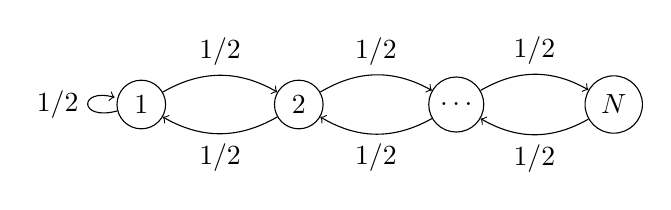
\begin{tikzpicture}[->,node distance=2cm]
                \node [circle,draw] (one) [] {1};
                \node [circle,draw] (two) [right of=one] {2};
                \node [circle,draw] (dots) [right of=two]{$\ldots$};
                \node [circle,draw] (enne) [right of=dots] {$N$};
                \path (one) edge [bend left] node [above] {1/2} (two);
                \path (two) edge [bend left] node [above] {1/2} (dots);
                \path (dots) edge [bend left] node [above] {1/2} (enne);
                \path (enne) edge [bend left] node [below] {1/2} (dots);
                \path (dots) edge [bend left] node [below] {1/2} (two);
                \path (two) edge [bend left] node [below] {1/2} (one);
                \path (one) edge [loop left] node [left] {1/2} (one);
            \end{tikzpicture}
    \label{symmrw}
\end{figure} whose invariant $\pi$ is the uniform on on $S_0$. Let $\tau$ be a finite random time on $\N$, independent of $Y$, such that:
\[
X_n=\begin{cases}
    Y_n &n<\tau\\
    0 &n>\tau
\end{cases}.
\]
So, in $\tau$, $X$ jumps to 0 and there remains. The transition probabilities are:
\[
i \in S_0:\;p_{ij}^{(n)}=\underbrace{\begin{cases}
    \prob(\tau=n)&j=0\\
    \frac{1}{2}(1-\prob(\tau-n)) &j=i\pm 1
\end{cases}}_{\text{there are called \textit{modulo boundaries}}}
\]
Since $\tau$ is independent, we have 
\begin{align*}
    \prob_{\pi}(X_n=i|\tau>n)&=\prob_{\pi}(X_n=i|X_n\neq0)\\
    &=\prob_{\pi}(Y_n=i)=\Pi_i
\end{align*}
\end{example}
\subsection{Hidden Markov Chains}
Hidden Markov Chains are a widely applied statistical framework, useful whenever it is necessary to estimate the current status of a system based on noisy or incomplete observations.

\textbf{Examples}:\begin{itemize}
    \item $X_n$: position of a moving object;\\
    $Y_n$: noisy observations of the position (by means, for instance, of a radar or a sonar);
    \item $X_n$: state of a productive system (that can be good or bad);\\
    $Y_n$: conditions of the output (that can be perfect or faulty);
    \item $X_n$: latent level of volatility in a financial market (high or low);\\
    $Y_n$: amount of financial products exchanged;
    \item $X_n$: number of alleles of type 0 in a population;\\
    $Y_n$: number of alleles of type 0 in a sample;
\end{itemize}
Let $X\sim Markov(\lambda, P)$ be unobserved (or hidden). This chain is sometimes called \textit{signal}. Every time $X$ enters a sate, an observation $Y$ (that we assume discrete on $\{a_1, a_2,\ldots\}$) is emitted with probability that depends on the current state of $X$ only. The model is:
\begin{align*}
    &\diamond \prob(X_n=j|X_{n-1}+i)=p_{ij}\\
    &\diamond \prob(\underbrace{Y_n=y_n}_{\mathclap{\text{generic realization of }Y}}|X_n=j)=p_j(y_n)
\end{align*}
$p_j(y_n)$ is the \textbf{emission distribution}, that is the likelihood of observing $Y_n$ if $X$ is in $j$. If $S+\{0,1\}$:
\begin{figure}[H]
    \centering
    \begin{tikzpicture}[->,>=stealth', line width=0.5pt, node distance=2cm]
        \node [circle,draw] (0) [] {0};
        \node [circle,draw] (a1) [below left=1.5cm and 0.2 cm of 0] {$a_1$};
        \node [circle,draw] (a2) [below right=1.5cm and 0.2 cm of 0]{$a_2$};
        \node [circle,draw] (1) [above right=1.5cm and 0.2 cm of a2] {1};
        \node [circle,draw] (a3) [below right=1.5cm and 0.2 cm  of 1] {$a_3$};
        \path (0) edge [black] node [above,midway,sloped] {\footnotesize$p_0(a_1)$} (a1);
        \path (0) edge [black] node [above,near end,sloped, rotate=180] {\footnotesize$\ldots$} (a2);
        \path (0) edge [black] node [above,near end,sloped, rotate=180] {\footnotesize$\ldots$} (a3);
        \path (1) edge [RedViolet] node [RedViolet,above,midway,sloped] {\footnotesize$p_1(a_3)$} (a3);
        \path (1) edge [RedViolet] node [RedViolet,above,near start,sloped, rotate=180] {\footnotesize$\ldots$} (a2);
        \path (1) edge [RedViolet] node [RedViolet,above,near start,sloped, rotate=180] {\footnotesize$\ldots$} (a1);
        \path (0) edge [bend left] node {} (1);
        \path (1) edge [bend left] node {} (0);
        \path (0) edge [loop left] node {} (0);
        \path (1) edge [loop right] node {} (1);
    \end{tikzpicture}
    \label{hidden}
\end{figure}
An alternative depiction is:
\begin{figure}[H]
    \centering
       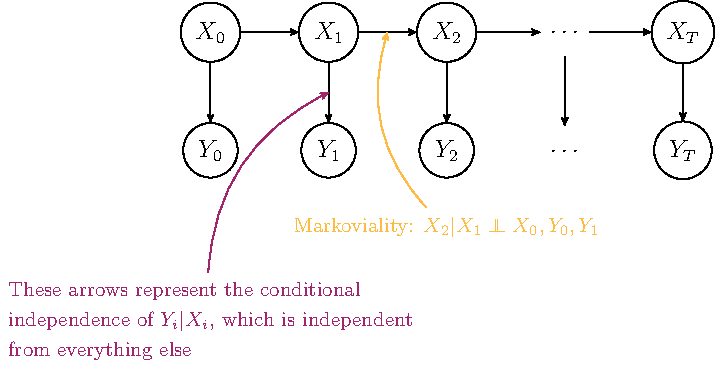
\includegraphics{../standalones/pdfs/hid}
    \label{hiddalt}
\end{figure}
The goal is to establish
\begin{align*}
    &\prob(X_{0:T}|Y_{0:T})\\
    \text{with}\quad &X_{0:T}=(X_0,\ldots,X_T)\\
    &Y_{0:T}=(Y_0,\ldots,Y_T)
\end{align*}
as the probability of a certain sequence of states of the system, given a sequence of observations. We can use the chain rule to write:
\[
\prob(X_T|Y_{0:T})\prob(X_{T-1}|X_T,Y_{0:T})\cdot\ldots\cdot\prob(X_0|X_{1:T},Y_{0:T})
\]
as the backwards decomposition. The generic factor is:
\begin{equation*}
    \prob(X_n|X_{n+1:T},Y_{0:T})=\prob(\underbrace{X_n|Y_{0:T}}_{\mathclap{Z}},\underbrace{X_{n+1}}_{W})
\end{equation*}
by virtue of the fact that $X_n|X_{n+1:T}\perp X_{n+2:T},Y_{n+1:T}$. By Bayes' theorem:
\begin{align*}
    \prob(Z|W)&\propto\prob(Z)\prob(W|Z)\\
    &\propto\prob(X_n|Y_{0:n})\prob(X_{n+1}|X_n,Y_{0:n})\\
    &=\prob(X_n|Y_{0:n})\prob(X_{n+1}|X_n)
\end{align*}
Since $X_{n+1}|X_n$ is independent from everything. $\prob(X_n|Y_{0:n})$ is the \textbf{filtering distribution}, the conditional law of $X$ given the information of past and present data, while $\prob(X_{n+1}|X_n)$ is the transition probability of $X$. \\Define
\[F_n(j)=\prob(X_n=j,Y_{0:n})\] so that
\[
\prob(X_n|Y_{0:n})=\frac{F_n(j)}{\sum_i F_n(i)}.
\]
Then
\begin{align*}
    F_n(j)&=\prob(Y_{0:n-1},X_n=j,Y_n=y_n)\\
    &=\sum_i\prob(\underbrace{Y_{0:n-1},X_{n-1}=i}_{F_{n-1}(i)},X_n=j,Y_n=y_n)\\
    &=\sum_i F_{n-1}(i)\underbrace{\prob(X_n=j,Y_n=y_n|X_{n-1}=i,Y_{0:n-1})}_{\prob(X_n|X_{n-1})\prob(Y_n|X_n)}\\
    &=\sum_i F_{n-1}(i)p_{ij}p_j(y_n)\\
    &\implies F_n(j)+\Bigl(\sum_iF_{n-1}(i)p_{ij}\Bigr)p_j(y_n)
\end{align*}
So that these can be computed recursively.
\begin{align*}
    F_0(j)&=\prob(X_0=j,Y_0)=\lambda_jp_j(y_0)\\
    F_1(j)&=\sum_i F_0(i)p_{ij}p_j(y_1)\\
    &=p_j(y_1)\sum_i\lambda_i p_i(y_0)p_{ij}
\end{align*}
If $S$ is finite, we can compute these quantities. Normalizing, we get the filtering distribution
\[
\prob(X_n=j|Y_{0:n})=\frac{F_n(j)}{\sum_i F_n(i)}.
\]
Moreover, if we consider the \textbf{marginal smoothing distribution}
\begin{align*}
    \prob(X_n|y_{0:n})&=\prob(\underbrace{X_n|Y_{0:n}}_{Z},\underbrace{Y_{n+1:T}}_{W})\\
    &\propto\prob(Z)\prob(W|Z)\qquad\text{since }Y_{n+1:T}|X_n \independent Y_{0:n}\\
    &=\underbrace{\prob(X_n|Y_{0:n})}_{\mathclap{\text{filtering distribution}}}\overbrace{\prob(Y_{n+1:T}|X_n)}^{\mathclap{B_n(\cdot)}}.
\end{align*}
$B_n(\cdot)$ is the \textbf{cost-to-go} function: it measures the likelihood of the future observations given a state of $X$:
\[B_n(j)+\prob(Y_{n+1:T}|X_n=j)\]
with
\[
\prob(X_n|Y_{0:T})\propto F_n(j)B_n(j).
\]
Also, $B_n$ can be computed recursively as
\[B_n(j)=\sum_i p_{ij}p_{j}(y_{n+1})B_{n+1}(j)\]
starting from $T$ and proceeding backwards. Finally, with these we have
\[
\prob(Y_{0:T})=\sum_jF_n(j)B_n(j)
\]
which represents the likelihood of the observations, which in principle can be maximized.
\subsection{General state space}
Assume for simplicity that $S\subset\R$ or $\R^k$ (uncountable). Define a time-homogeneous transition probability from 
\[\prob(x,A):=\prob(X_{n+1}\in A|X_n=x),\qquad A\in\mathscr{B}(S).\]
If this has a density with respect to some dominant measure $\nu$, we call
\[p=\frac{dP}{d\nu}\]
the \textbf{transition density}.\\
For example, if $\nu$ is the Lebesgue measure,
\[\prob(x,A)=\int_A \prob(x.y)dy\].
\begin{definition}
    A Markov Chain o $S$ uncountable is said to be $\mathbf{\varphi}$\textbf{-irreducible} if there exists a $\sigma$-finite measure $\varphi$ on $S$ such that $\forall A\in\mathscr{B}(S)$ with $\varphi(A)>0$ and for all $x\in S\;\exists\geqslant1,\;n=n(x,A)$ such that $p^{(n)}(x,A)>0$.
\end{definition}
\begin{definition}
    A $\varphi$-irreducible Markov Chain is said to be \textbf{Harris Recurrent} if $\forall A \in \mathscr{B}(S)$ such that $\varphi(A)>0$ then $\prob(X_n\in A \text{ i.o.})=1$. It is called \textit{positive} if it admits an invariant distribution $\pi$.
\end{definition}
$\pi$ is invariant if $\int_A\pi(dx)p(x,dy)=\pi(A)$.
\begin{theorem}
    Let $X$ be aperiodic and positive Harris recurrent. Then
        \[d_{TV}(\lambda P^n,\pi)\xrightarrow[n\to\infty]{}0
        \]
        where
        \begin{itemize}
            \item $\displaystyle\lambda P^n(A)=\int\limits_SP^n(x,A)\lambda(dx)$
            \item $\displaystyle d_{TV}(\lambda,\mu)=\sup\limits_{A\in\mathscr{B}}|\prob(V\in A)-\prob(W\in A)|$ if $V\sim\lambda$ and $W\sim\mu$.
        \end{itemize}
        If, in addition, $f:S\to\R$ is $\pi$-integrable
        \[
        \frac{1}{N}\sum_{i=1}^Nf(X_n)\xrightarrow[N\to\infty]{}\int_Sf(x)\pi(dx)
        \]
        with probability 1.
\end{theorem}
\begin{definition}
    Let $X$ be aperiodic and positive Harris recurrent. Then
        \[d_{TV}(\lambda P^n,\pi)\xrightarrow[n\to\infty]{}0
        \]
        where
        \begin{itemize}
            \item $\displaystyle\lambda P^n(A)=\int\limits_SP^n(x,A)\lambda(dx)$
            \item $\displaystyle d_{TV}(\lambda,\mu)=\sup\limits_{A\in\mathscr{B}}|\prob(V\in A)-\prob(W\in A)|$ if $V\sim\lambda$ and $W\sim\mu$.
        \end{itemize}
        If, in addition, $f:S\to\R$ is $\pi$-integrable
        \[
        \frac{1}{N}\sum_{i=1}^Nf(X_n)\xrightarrow[N\to\infty]{}\int_Sf(x)\pi(dx)
        \]
        with probability 1.
\end{definition}
\begin{figure}[H]
    \centering
    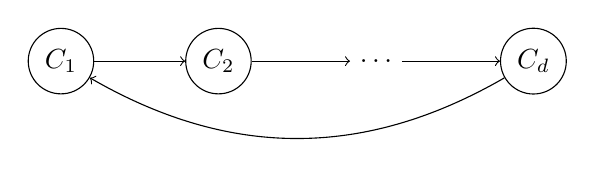
\begin{tikzpicture}[->,node distance=2cm]
        \node[circle, draw](c1){$C_1$};
        \node[circle,draw](c2)[right of=c1]{$C_2$};
        \node[](dots)[right of=c2]{$\ldots$};
        \node[circle,draw](cd)[right of=dots]{$C_d$};
        \path (c1) edge (c2);
        \path (c2) edge (dots);
        \path (dots) edge (cd);
        \path (cd) edge [bend left] (c1);
    \end{tikzpicture}
    \label{dperiod}
\end{figure}
\end{document}